\section{Chiusure}
Come gi\`a osservato nell'esempio introduttivo, il modello botton-up su una rete richiede un elevato numero di equazioni differenziali: le equazioni per i nodi dipendono dalle coppie, le coppie dalle triple e cos\`i via.\\
Tale approccio, al crescere del numero di nodi, risulterebbe computazionalmente intrattabile. Per risolvere questo problema dobbiamo trovare alcune semplificazioni che ci permettano di esprimere le coppie in termini dei singoli nodi, le triple in termini delle coppie e dei nodi e cos\`i via.\\
Se riusciamo a fare ci\`o, possiamo rompere la ``cascata" nella quale ogni struttura dipende da tutte le strutture di ordine superiore.\\ \\
Andiamo a presentare un approccio formale basato sul lavoro di Keeling~\cite{keeling1995ecology}  e van Baalen~\cite{van2000pair}.  A tal fine introduciamo i  \textit{coefficienti di correlazione}.\\
Siano $A, B\in \{ S, I,R\}$ e $(i,j)\in E$ allora 
$$C_{A_i B_j} = \frac{\angol{A_i B_j}}{\angol{A_i} \angol{B_j}}.$$
Tali coefficienti quantificano la propensione che due nodi adiacenti abbiamo stato differente o identico.\\
Se $C_{A_iB_j}=1$ allora possiamo, in modo equivalente, assuemere  $A_i$ e $B_j$ indipendenti.\\
Osserviamo che nel modello $SIR$ gli stati non sono per\`o indipendenti. I nodi infetti possono infettare i loro vicini dunque hanno una maggior probabilit\`a di essere uniti ad altri nodi infetti,  di conseguenza  $C_{I_i I_j}\geq 1$.  Diremo che $I_i$ e $I_j$ sono correlati positivamente.\\
Con medesime argomentazioni si arriva a dire che $S_i$ e $I_j$ sono correlati negativamente: $C_{S_i I_j}\leq 1$.\\
 In un certo senso, sapere che $j$ \`e infetto aumenta la nostra aspettativa  che $i$ sia infetto e diminuisce quella che sia sano.\\
 
\subsection{Chiusura al livello delle coppie}
Da quanto osservato nella parte introduttiva sulle chiusure, possiamo scrivere:
$$ \angol{ A_i B_j} = \angol{ A_i} \angol{B_j} C_{A_i B_j} \text{ dove } A,B\in \{S,I,R\} \text{ e } (i,j)\in E.$$ 
Assumendo, in prima approssimazione, l'indipendenza a livello delle coppie abbiamo 
$$ \angol{ A_i B_j} \approx \angol{A_i}\angol{B_j}.$$ 
Per enfatizzare che non abbiamo identit\`a esatte, quando andremo a risolvere un sistema ottenuto usando le chiusure denoteremo  con $\angol{X_i}$ l'approssimazione di $\angol{ S_i}$ e con $\angol{ Y_i}$ quella di $\angol{ I_i}$.\\ \\
Presentiamo il modello botton-up generale su una rete con $N$ nodi senza loop e mostriamo come usando l'indipendenza a livello delle coppie si riesca ad ottenere un sistema di equazioni differenziali chiuse.\\
Sia $G=(g_{ij})$ la matrice di adiacenza del grafo $G$. Assumiamo che il tasso di trasmissione da $i$ a $j$ sia $\tau g_{ij}$ e che il tasso di rimozione per il nodo $i$ sia $\gamma_i$ indipendentemente dallo stato di ogni altro nodo.\\
Dunque le equazione per il sistema diventano
\begin{equation}
\begin{aligned}
	 \angol{ S_i} =& - \sum_{j=1\atop{j\neq i }}^N g_{ij} \angol{ S_i I_j},\\
	 \angol{I_i} =&\spa \tau \sum_{j=1\atop{j\neq i}}^N  g_{ij} \angol{ S_i I_j} -\gamma_i \angol{I_i},
\end{aligned}
\end{equation}
dove ricordiamo che $\angol{R_i}=1-\angol{S_i}- \angol{I_i}$.\\
Usando l'indipendenza a livello delle coppie possiamo un sistema chiuso: 
\begin{equation}
\begin{aligned}
	 \angol{ X_i} =& -\tau \sum_{j=1\atop{j\neq i }}^N g_{ij}\angol{ X_i} \angol{Y_j},\\
	 \angol{Y_i} =&\spa \tau \sum_{j=1\atop{j\neq i}}^N  g_{ij}\angol{ X_i}\angol{Y_j} -\gamma_i \angol{Y_i}.
\end{aligned}
\label{Coppie3nodi}
\end{equation}
Possiamo scrivere il sistema precedente in forma vettoriale:
\begin{equation}
	\begin{aligned}
	\dot{\angol{X}} = & - \tau G X * Y,\\
	\dot{\angol{Y}}=& \spa \tau G X * Y - \Gamma Y,	
	\end{aligned}
\end{equation}
dove $\Gamma=diag(\gamma_1, \dots, \gamma_n)$ e il prodotto tra vettori \`e inteso elemento per elemento.\\

Nella Figura~\ref{fig::coppie3nodi} possiamo confrontare le soluzioni del modello esatto con l'approssimazione ottenuta  dall'indipendenza a livello delle coppie per il grafo~\ref{fig::3nodi}. Per non appesantire i grafici abbiamo tracciato solamente  $\angol{S_i}$ e $\angol{I_i}$ in funzione  del tempo: $\angol{ R_i}$ pu\`o essere ricavata.\\
Dalla Figura~\ref{fig::coppie3nodi} (d) possiamo notare che il modello semplificato tende a sottostimare la prevalenza della malattia. Tale sottostima risulta sconveniente se volessimo usare queste  predizioni per intervenire con delle politiche di contenimento. Nelle sezioni successive ci domanderemo se sia possibile trovare una rappresentazione con un numero minore di variabili che sia pi\`u accurato o, meglio ancora esatta.  \begin{figure}[!h]

\centering
\subfloat[][Nodo 1]
{\resizebox{0.45\textwidth}{!}{% This file was created by matlab2tikz.
%
%The latest updates can be retrieved from
%  http://www.mathworks.com/matlabcentral/fileexchange/22022-matlab2tikz-matlab2tikz
%where you can also make suggestions and rate matlab2tikz.
%
\begin{tikzpicture}

\begin{axis}[%
width=6.028in,
height=4.754in,
at={(1.011in,0.642in)},
scale only axis,
xmin=0,
xmax=5,
ymin=0,
ymax=1,
axis background/.style={fill=white},
axis x line*=bottom,
axis y line*=left,
legend style={legend cell align=left, align=left, draw=white!15!black}
]
\addplot [color=blue, dashed, line width=2.0pt]
  table[row sep=crcr]{%
0	0\\
0.000100475457260383	0\\
0.000200950914520766	0\\
0.00030142637178115	0\\
0.000401901829041533	0\\
0.000904279115343449	0\\
0.00140665640164536	0\\
0.00190903368794728	0\\
0.0024114109742492	0\\
0.00492329740575878	0\\
0.00743518383726836	0\\
0.00994707026877794	0\\
0.0124589567002875	0\\
0.0250183888578354	0\\
0.0375778210153833	0\\
0.0501372531729312	0\\
0.0626966853304791	0\\
0.0991412937643315	0\\
0.135585902198184	0\\
0.172030510632036	0\\
0.208475119065889	0\\
0.257093885813804	0\\
0.305712652561719	0\\
0.354331419309635	0\\
0.40295018605755	0\\
0.46627950019307	0\\
0.52960881432859	0\\
0.592938128464109	0\\
0.656267442599629	0\\
0.733658471248229	0\\
0.811049499896829	0\\
0.888440528545428	0\\
0.965831557194028	0\\
1.05793596976172	0\\
1.15004038232942	0\\
1.24214479489711	0\\
1.3342492074648	0\\
1.44286725998794	0\\
1.55148531251107	0\\
1.66010336503421	0\\
1.76872141755734	0\\
1.88893196521442	0\\
2.00914251287149	0\\
2.12935306052856	0\\
2.24956360818563	0\\
2.37456360818563	0\\
2.49956360818563	0\\
2.62456360818563	0\\
2.74956360818563	0\\
2.87456360818563	0\\
2.99956360818563	0\\
3.12456360818563	0\\
3.24956360818563	0\\
3.37456360818563	0\\
3.49956360818563	0\\
3.62456360818563	0\\
3.74956360818563	0\\
3.87456360818563	0\\
3.99956360818563	0\\
4.12456360818563	0\\
4.24956360818563	0\\
4.37456360818563	0\\
4.49956360818563	0\\
4.62456360818563	0\\
4.74956360818563	0\\
4.81217270613922	0\\
4.87478180409282	0\\
4.93739090204641	0\\
5	0\\
};
\addlegendentry{$\langle\text{ S}_\text{1}\rangle\text{(t)}$}

\addplot [color=blue, dashdotted, line width=2.0pt]
  table[row sep=crcr]{%
0	1\\
0.000100475457260383	0.999899530851975\\
0.000200950914520766	0.999799074321068\\
0.00030142637178115	0.999698630405252\\
0.000401901829041533	0.999598199102498\\
0.000904279115343449	0.999096231713726\\
0.00140665640164536	0.998594579347576\\
0.00190903368794728	0.998093241751005\\
0.0024114109742492	0.997592218671205\\
0.00492329740575878	0.995091812191547\\
0.00743518383726836	0.992599230844247\\
0.00994707026877794	0.99011444329054\\
0.0124589567002875	0.987637418335814\\
0.0250183888578354	0.975367649924921\\
0.0375778210153833	0.963287349850503\\
0.0501372531729312	0.95139277818569\\
0.0626966853304791	0.939680278465966\\
0.0991412937643315	0.906691121197265\\
0.135585902198184	0.875122026261053\\
0.172030510632036	0.84489505392913\\
0.208475119065889	0.815936847771523\\
0.257093885813804	0.779162082786105\\
0.305712652561719	0.744374033314346\\
0.354331419309635	0.711435438681249\\
0.40295018605755	0.680218977306833\\
0.46627950019307	0.641947443142085\\
0.52960881432859	0.606170880086586\\
0.592938128464109	0.57268300941166\\
0.656267442599629	0.541294639807272\\
0.733658471248229	0.505539700874787\\
0.811049499896829	0.472401400098227\\
0.888440528545428	0.441643779926677\\
0.965831557194028	0.413050790490989\\
1.05793596976172	0.381577729092981\\
1.15004038232942	0.352633357286117\\
1.24214479489711	0.32598137605421\\
1.3342492074648	0.301403668240138\\
1.44286725998794	0.274823389324357\\
1.55148531251107	0.250608123714557\\
1.66010336503421	0.228532043064533\\
1.76872141755734	0.208383481405329\\
1.88893196521442	0.18810670108475\\
2.00914251287149	0.169761602533511\\
2.12935306052856	0.153164227225967\\
2.24956360818563	0.138140887512441\\
2.37456360818563	0.124022366485792\\
2.49956360818563	0.111296789759966\\
2.62456360818563	0.0998320653432603\\
2.74956360818563	0.0895042491653371\\
2.87456360818563	0.0802017913363273\\
2.99956360818563	0.0718297511966022\\
3.12456360818563	0.0642998582961289\\
3.24956360818563	0.0575300406300992\\
3.37456360818563	0.0514459189750346\\
3.49956360818563	0.0459824167257564\\
3.62456360818563	0.0410795185781667\\
3.74956360818563	0.0366818144806219\\
3.87456360818563	0.0327390432193454\\
3.99956360818563	0.0292067909974307\\
4.12456360818563	0.026044356733585\\
4.24956360818563	0.0232143512207873\\
4.37456360818563	0.0206829253611926\\
4.49956360818563	0.0184201426618039\\
4.62456360818563	0.0163986992689843\\
4.74956360818563	0.0145936013829732\\
4.81217270613922	0.0137636454521629\\
4.87478180409282	0.0129797303849961\\
4.93739090204641	0.0122393928316829\\
5	0.0115402885602625\\
};
\addlegendentry{$\langle\text{ I}_\text{1}\rangle\text{(t)}$}

\addplot [color=red, dashed, line width=2.0pt]
  table[row sep=crcr]{%
0	0\\
0.000100475457260383	0\\
0.000200950914520766	0\\
0.00030142637178115	0\\
0.000401901829041533	0\\
0.000904279115343449	0\\
0.00140665640164536	0\\
0.00190903368794728	0\\
0.0024114109742492	0\\
0.00492329740575878	0\\
0.00743518383726836	0\\
0.00994707026877794	0\\
0.0124589567002875	0\\
0.0250183888578354	0\\
0.0375778210153833	0\\
0.0501372531729312	0\\
0.0626966853304791	0\\
0.102108236390274	0\\
0.141519787450068	0\\
0.180931338509863	0\\
0.220342889569658	0\\
0.274870838360705	0\\
0.329398787151753	0\\
0.383926735942801	0\\
0.438454684733849	0\\
0.511698843017727	0\\
0.584943001301606	0\\
0.658187159585485	0\\
0.731431317869363	0\\
0.823962581336954	0\\
0.916493844804545	0\\
1.00902510827214	0\\
1.10155637173973	0\\
1.21569652246265	0\\
1.32983667318558	0\\
1.44397682390851	0\\
1.55811697463144	0\\
1.68311697463144	0\\
1.80811697463144	0\\
1.93311697463144	0\\
2.05811697463144	0\\
2.18311697463144	0\\
2.30811697463144	0\\
2.43311697463144	0\\
2.55811697463144	0\\
2.68311697463144	0\\
2.80811697463144	0\\
2.93311697463144	0\\
3.05811697463144	0\\
3.18311697463144	0\\
3.30811697463144	0\\
3.43311697463144	0\\
3.55811697463144	0\\
3.68311697463144	0\\
3.80811697463144	0\\
3.93311697463144	0\\
4.05811697463144	0\\
4.18311697463144	0\\
4.30811697463144	0\\
4.43311697463144	0\\
4.55811697463144	0\\
4.66858773097358	0\\
4.77905848731572	0\\
4.88952924365786	0\\
5	0\\
};
\addlegendentry{$\langle\text{ X}_\text{1}\rangle\text{(t)}$}

\addplot [color=red, dashdotted, line width=2.0pt]
  table[row sep=crcr]{%
0	1\\
0.000100475457260383	0.999899529590229\\
0.000200950914520766	0.999799069274762\\
0.00030142637178115	0.999698619052584\\
0.000401901829041533	0.99959817892268\\
0.000904279115343449	0.999096129621802\\
0.00140665640164536	0.998594332475746\\
0.00190903368794728	0.998092787357867\\
0.0024114109742492	0.997591494141582\\
0.00492329740575878	0.995088802158148\\
0.00743518383726836	0.992592388763919\\
0.00994707026877794	0.990102238207607\\
0.0124589567002875	0.987618334777361\\
0.0250183888578354	0.975291977237725\\
0.0375778210153833	0.963119463697323\\
0.0501372531729312	0.951098874131562\\
0.0626966853304791	0.93922831221879\\
0.102108236390274	0.902931778663981\\
0.141519787450068	0.868037944344166\\
0.180931338509863	0.834492632110179\\
0.220342889569658	0.802243674259999\\
0.274870838360705	0.759670071118651\\
0.329398787151753	0.719355843996611\\
0.383926735942801	0.681181236610769\\
0.438454684733849	0.645032460981824\\
0.511698843017727	0.599475695073584\\
0.584943001301606	0.557136712694367\\
0.658187159585485	0.517788820999762\\
0.731431317869363	0.481219878010058\\
0.823962581336954	0.438688408765387\\
0.916493844804545	0.399916524725773\\
1.00902510827214	0.364573468010499\\
1.10155637173973	0.332353956114381\\
1.21569652246265	0.296500561034228\\
1.32983667318558	0.26451591154939\\
1.44397682390851	0.23598602108473\\
1.55811697463144	0.210533572030706\\
1.68311697463144	0.185791792103997\\
1.80811697463144	0.163958587530347\\
1.93311697463144	0.144695683390095\\
2.05811697463144	0.12769628713977\\
2.18311697463144	0.112689495570161\\
2.30811697463144	0.0994468609939923\\
2.43311697463144	0.0877632073395494\\
2.55811697463144	0.0774524537440724\\
2.68311697463144	0.0683502875344955\\
2.80811697463144	0.0603181468596634\\
2.93311697463144	0.0532315849517043\\
3.05811697463144	0.046977736983156\\
3.18311697463144	0.0414569413272378\\
3.30811697463144	0.0365851551694901\\
3.43311697463144	0.0322868970080767\\
3.55811697463144	0.0284937102102783\\
3.68311697463144	0.0251451463659556\\
3.80811697463144	0.022190230444078\\
3.93311697463144	0.0195831801618519\\
4.05811697463144	0.0172824740757185\\
4.18311697463144	0.01525144802108\\
4.30811697463144	0.0134591837831516\\
4.43311697463144	0.0118779127382733\\
4.55811697463144	0.010482450617124\\
4.66858773097358	0.00938602881979297\\
4.77905848731572	0.00840431505031311\\
4.88952924365786	0.00752539974058104\\
5	0.00673840764530069\\
};
\addlegendentry{$\langle\text{ Y}_\text{1}\rangle\text{(t)}$}

\end{axis}
\end{tikzpicture}%}}
 \quad 
\subfloat[][Nodo 2]
{\resizebox{0.45\textwidth}{!}{ % This file was created by matlab2tikz.
%
%The latest updates can be retrieved from
%  http://www.mathworks.com/matlabcentral/fileexchange/22022-matlab2tikz-matlab2tikz
%where you can also make suggestions and rate matlab2tikz.
%
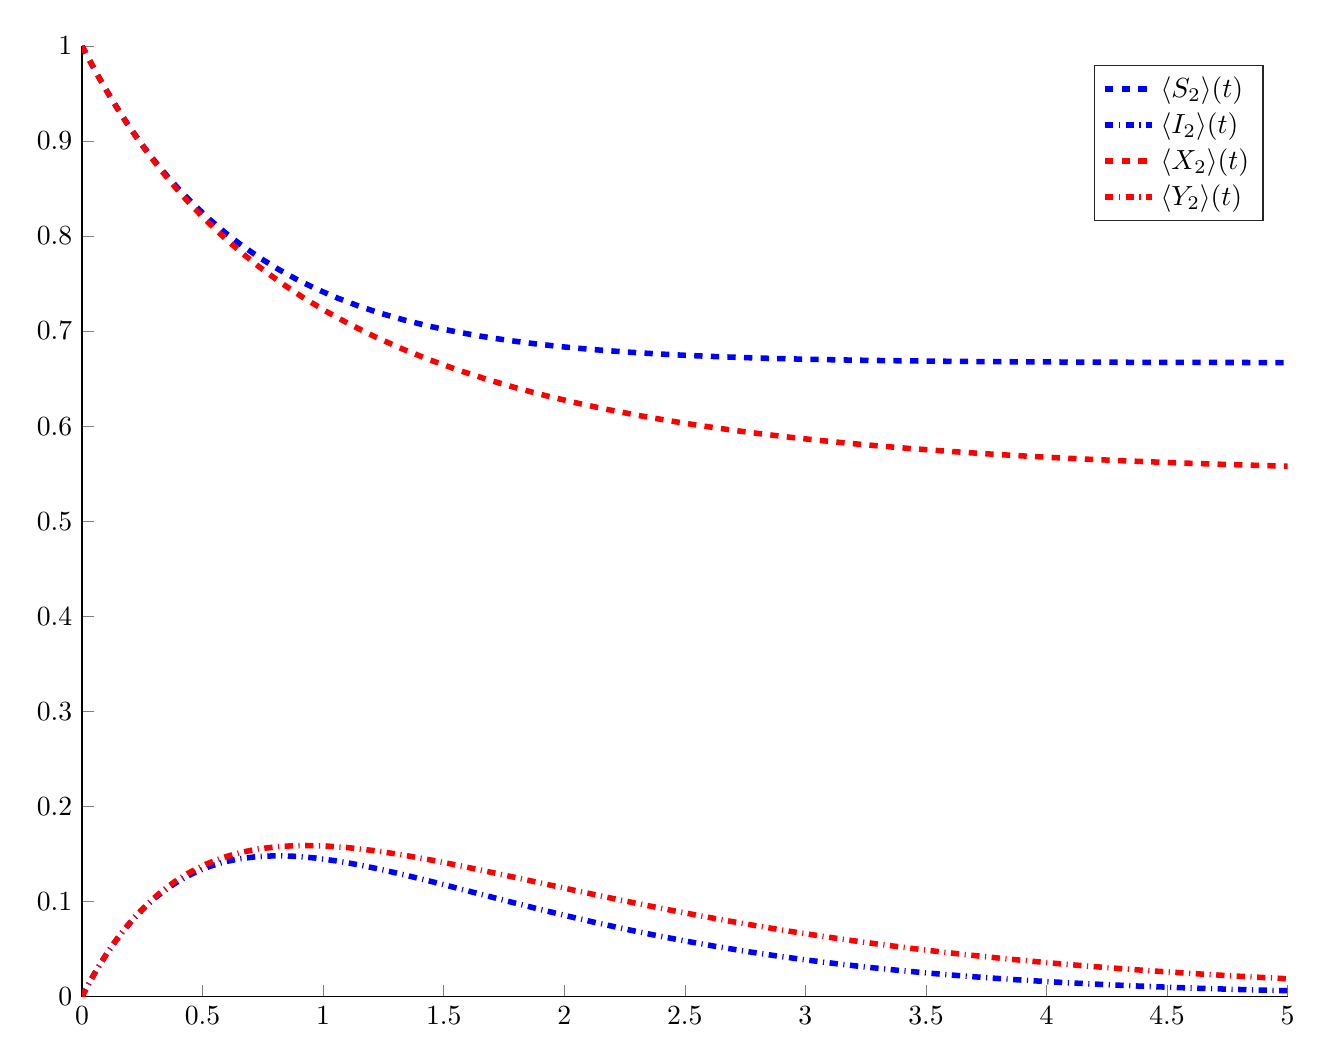
\begin{tikzpicture}

\begin{axis}[%
width=6.028in,
height=4.754in,
at={(1.011in,0.642in)},
scale only axis,
xmin=0,
xmax=5,
ymin=0,
ymax=1,
axis background/.style={fill=white},
axis x line*=bottom,
axis y line*=left,
legend style={legend cell align=left, align=left, draw=white!15!black}
]
\addplot [color=blue, dashed, line width=2.0pt]
  table[row sep=crcr]{%
0	1\\
0.000100475457260383	0.999949766056924\\
0.000200950914520766	0.999899539684195\\
0.00030142637178115	0.999849320880672\\
0.000401901829041533	0.999799109645214\\
0.000904279115343449	0.999548166948998\\
0.00140665640164536	0.999297413283416\\
0.00190903368794728	0.999046848506074\\
0.0024114109742492	0.998796472474686\\
0.00492329740575878	0.997547418534447\\
0.00743518383726836	0.996303061961732\\
0.00994707026877794	0.995063385091027\\
0.0124589567002875	0.993828370323048\\
0.0250183888578354	0.987722616365095\\
0.0375778210153833	0.981730813042634\\
0.0501372531729312	0.975850833944071\\
0.0626966853304791	0.970080591669277\\
0.0991412937643315	0.953939046011196\\
0.135585902198184	0.938656254473793\\
0.172030510632036	0.924186587013759\\
0.208475119065889	0.910486692796938\\
0.257093885813804	0.893338017841503\\
0.305712652561719	0.877395555845\\
0.354331419309635	0.862574680234777\\
0.40295018605755	0.848796177141757\\
0.46627950019307	0.832290618164177\\
0.52960881432859	0.817281114199863\\
0.592938128464109	0.803632751202841\\
0.656267442599629	0.791221205689014\\
0.733658471248229	0.777568429104202\\
0.811049499896829	0.765412570030883\\
0.888440528545428	0.754590931818442\\
0.965831557194028	0.744955370973288\\
1.05793596976172	0.734850994744874\\
1.15004038232942	0.726051284757239\\
1.24214479489711	0.718390163309227\\
1.3342492074648	0.711717689094676\\
1.44286725998794	0.704941359996623\\
1.55148531251107	0.699184906067961\\
1.66010336503421	0.694298310044978\\
1.76872141755734	0.690146590836533\\
1.88893196521442	0.68626979781265\\
2.00914251287149	0.683033580994597\\
2.12935306052856	0.680335328566429\\
2.24956360818563	0.678082495710856\\
2.37456360818563	0.676129062260638\\
2.49956360818563	0.67451015902841\\
2.62456360818563	0.673170462694345\\
2.74956360818563	0.672059963058475\\
2.87456360818563	0.6711370825968\\
2.99956360818563	0.670372247653384\\
3.12456360818563	0.669739321268742\\
3.24956360818563	0.669214676614722\\
3.37456360818563	0.668778670798171\\
3.49956360818563	0.66841733203559\\
3.62456360818563	0.668118312176992\\
3.74956360818563	0.667870448959301\\
3.87456360818563	0.66766446229043\\
3.99956360818563	0.667493751338391\\
4.12456360818563	0.667352482340913\\
4.24956360818563	0.667235381796357\\
4.37456360818563	0.667138065416295\\
4.49956360818563	0.667057414702439\\
4.62456360818563	0.666990673551059\\
4.74956360818563	0.666935350548061\\
4.81217270613922	0.666911265128768\\
4.87478180409282	0.666889339104704\\
4.93739090204641	0.666869379826172\\
5	0.66685120964227\\
};
\addlegendentry{$\langle\text{ S}_\text{2}\text{ }\rangle\text{(t)}$}

\addplot [color=blue, dashdotted, line width=2.0pt]
  table[row sep=crcr]{%
0	0\\
0.000100475457260383	5.02314194582358e-05\\
0.000200950914520766	0.000100450222178378\\
0.00030142637178115	0.000150656410568844\\
0.000401901829041533	0.000200849987037635\\
0.000904279115343449	0.000451628774807697\\
0.00140665640164536	0.00070209262549841\\
0.00190903368794728	0.000952241839644842\\
0.0024114109742492	0.00120207671752405\\
0.00492329740575878	0.00244654655480787\\
0.00743518383726836	0.00368320287872335\\
0.00994707026877794	0.00491208293452641\\
0.0124589567002875	0.0061332238082172\\
0.0250183888578354	0.0121241281424412\\
0.0375778210153833	0.0179270245694221\\
0.0501372531729312	0.0235463722993485\\
0.0626966853304791	0.02898653721096\\
0.0991412937643315	0.0437975780064231\\
0.135585902198184	0.0572353494401202\\
0.172030510632036	0.0693937083334257\\
0.208475119065889	0.0803611576950339\\
0.257093885813804	0.0932814625263713\\
0.305712652561719	0.104411444050903\\
0.354331419309635	0.113918297020974\\
0.40295018605755	0.121956876117229\\
0.46627950019307	0.130459773511127\\
0.52960881432859	0.13699148818833\\
0.592938128464109	0.141802573766275\\
0.656267442599629	0.145120569742411\\
0.733658471248229	0.147443262414491\\
0.811049499896829	0.148152783459638\\
0.888440528545428	0.147523537737773\\
0.965831557194028	0.145800614492561\\
1.05793596976172	0.14261761324062\\
1.15004038232942	0.138468469319266\\
1.24214479489711	0.133593199535327\\
1.3342492074648	0.128203232510097\\
1.44286725998794	0.121423706047034\\
1.55148531251107	0.114375584460389\\
1.66010336503421	0.10722364787831\\
1.76872141755734	0.100112083509218\\
1.88893196521442	0.0924224291243308\\
2.00914251287149	0.0850002476399585\\
2.12935306052856	0.0779076868343403\\
2.24956360818563	0.0711991011319526\\
2.37456360818563	0.0646673812660732\\
2.49956360818563	0.0585888424369925\\
2.62456360818563	0.0529600282470089\\
2.74956360818563	0.0477773110138708\\
2.87456360818563	0.0430297403451633\\
2.99956360818563	0.0386916182635999\\
3.12456360818563	0.0347385923849993\\
3.24956360818563	0.0311483438435658\\
3.37456360818563	0.0278975046540668\\
3.49956360818563	0.0249585909052709\\
3.62456360818563	0.0223063173817782\\
3.74956360818563	0.0199176420689963\\
3.87456360818563	0.0177704893156483\\
3.99956360818563	0.0158425684352806\\
4.12456360818563	0.0141135755002288\\
4.24956360818563	0.0125650442349459\\
4.37456360818563	0.0111798516748117\\
4.49956360818563	0.00994182226490993\\
4.62456360818563	0.0088362940755339\\
4.74956360818563	0.00784994516657192\\
4.81217270613922	0.00739687025071491\\
4.87478180409282	0.00696920095174279\\
4.93739090204641	0.00656558347103006\\
5	0.00618472765868362\\
};
\addlegendentry{$\langle\text{ I}_\text{2}\rangle\text{(t)}$}

\addplot [color=red, dashed, line width=2.0pt]
  table[row sep=crcr]{%
0	1\\
0.000100475457260383	0.99994976605686\\
0.000200950914520766	0.999899539683687\\
0.00030142637178115	0.999849320878961\\
0.000401901829041533	0.999799109641159\\
0.000904279115343449	0.99954816690284\\
0.00140665640164536	0.999297413109794\\
0.00190903368794728	0.999046848072382\\
0.0024114109742492	0.998796471601204\\
0.00492329740575878	0.997547411126232\\
0.00743518383726836	0.996303036533294\\
0.00994707026877794	0.995063324412706\\
0.0124589567002875	0.993828251500648\\
0.0250183888578354	0.987721670488083\\
0.0375778210153833	0.981727662789085\\
0.0501372531729312	0.975843478285104\\
0.0626966853304791	0.970066449874119\\
0.102108236390274	0.952605420168752\\
0.141519787450068	0.936099675314657\\
0.180931338509863	0.920480826836349\\
0.220342889569658	0.905686357257161\\
0.274870838360705	0.886471518613129\\
0.329398787151753	0.868591348141757\\
0.383926735942801	0.851925610206075\\
0.438454684733849	0.836366826263978\\
0.511698843017727	0.81704354767056\\
0.584943001301606	0.799345706541171\\
0.658187159585485	0.783098638750895\\
0.731431317869363	0.76814911627258\\
0.823962581336954	0.750913024428527\\
0.916493844804545	0.735311720644982\\
1.00902510827214	0.721151661167631\\
1.10155637173973	0.708264369444304\\
1.21569652246265	0.693908865254259\\
1.32983667318558	0.681051271536474\\
1.44397682390851	0.669502958947782\\
1.55811697463144	0.659099610029634\\
1.68311697463144	0.648856496917941\\
1.80811697463144	0.639673519417067\\
1.93311697463144	0.631422907332402\\
2.05811697463144	0.62399201116677\\
2.18311697463144	0.617284880263026\\
2.30811697463144	0.611222776938041\\
2.43311697463144	0.605735753729153\\
2.55811697463144	0.600761252574241\\
2.68311697463144	0.596244823027247\\
2.80811697463144	0.592140568132477\\
2.93311697463144	0.588407274158174\\
3.05811697463144	0.585007690098468\\
3.18311697463144	0.581908882003535\\
3.30811697463144	0.579082536837936\\
3.43311697463144	0.576503021741188\\
3.55811697463144	0.574146990158659\\
3.68311697463144	0.571993567402675\\
3.80811697463144	0.570024546403732\\
3.93311697463144	0.56822334343106\\
4.05811697463144	0.566574770310173\\
4.18311697463144	0.565065136603473\\
4.30811697463144	0.563682374949081\\
4.43311697463144	0.562415445174647\\
4.55811697463144	0.561254196069616\\
4.66858773097358	0.56030851506375\\
4.77905848731572	0.559432507092414\\
4.88952924365786	0.558620902201171\\
5	0.557868805996139\\
};
\addlegendentry{$\langle\text{ X}_\text{2}\rangle\text{(t)}$}

\addplot [color=red, dashdotted, line width=2.0pt]
  table[row sep=crcr]{%
0	0\\
0.000100475457260383	5.02314195216212e-05\\
0.000200950914520766	0.000100450222685378\\
0.00030142637178115	0.00015065641227969\\
0.000401901829041533	0.000200849991092313\\
0.000904279115343449	0.000451628820955347\\
0.00140665640164536	0.000702092799059145\\
0.00190903368794728	0.000952242273129502\\
0.0024114109742492	0.00120207759047991\\
0.00492329740575878	0.00244655395390654\\
0.00743518383726836	0.00368322825984696\\
0.00994707026877794	0.00491214346181296\\
0.0124589567002875	0.00613334226017403\\
0.0250183888578354	0.0121250680925129\\
0.0375778210153833	0.0179301450594698\\
0.0501372531729312	0.023553635330364\\
0.0626966853304791	0.0290004563591362\\
0.102108236390274	0.044998106770484\\
0.141519787450068	0.0594409659043847\\
0.180931338509863	0.0724560696360787\\
0.220342889569658	0.0841600869174819\\
0.274870838360705	0.0983885821787152\\
0.329398787151753	0.110563341086724\\
0.383926735942801	0.120909930751128\\
0.438454684733849	0.129630673618899\\
0.511698843017727	0.139099340842715\\
0.584943001301606	0.14633229027685\\
0.658187159585485	0.151654455741052\\
0.731431317869363	0.155350568031261\\
0.823962581336954	0.158073528446468\\
0.916493844804545	0.158994675694103\\
1.00902510827214	0.158455276740108\\
1.10155637173973	0.15674915749057\\
1.21569652246265	0.153397558084643\\
1.32983667318558	0.148992022221842\\
1.44397682390851	0.14381988595314\\
1.55811697463144	0.138124909820625\\
1.68311697463144	0.131515619398056\\
1.80811697463144	0.124686585141643\\
1.93311697463144	0.117780309428003\\
2.05811697463144	0.110915874064973\\
2.18311697463144	0.10418236746683\\
2.30811697463144	0.097633998120614\\
2.43311697463144	0.0913133288412923\\
2.55811697463144	0.0852540775432535\\
2.68311697463144	0.0794782645069583\\
2.80811697463144	0.0739939269600281\\
2.93311697463144	0.068804964989228\\
3.05811697463144	0.0639123325840836\\
3.18311697463144	0.0593127662216291\\
3.30811697463144	0.0549977514099881\\
3.43311697463144	0.0509577192898392\\
3.55811697463144	0.0471825185717931\\
3.68311697463144	0.0436608459305459\\
3.80811697463144	0.0403798026923218\\
3.93311697463144	0.0373266305829282\\
4.05811697463144	0.0344888684754468\\
4.18311697463144	0.0318541013086588\\
4.30811697463144	0.0294097888400823\\
4.43311697463144	0.027143921496779\\
4.55811697463144	0.025045044993035\\
4.66858773097358	0.02332031744584\\
4.77905848731572	0.0217100684354412\\
4.88952924365786	0.0202073223544393\\
5	0.0188054435162205\\
};
\addlegendentry{$\langle\text{ Y}_\text{2}\rangle\text{(t)}$}

\end{axis}
\end{tikzpicture}%}}
\\
\subfloat[][Nodo 3]
{\resizebox{0.45\textwidth}{!}
{% This file was created by matlab2tikz.
%
%The latest updates can be retrieved from
%  http://www.mathworks.com/matlabcentral/fileexchange/22022-matlab2tikz-matlab2tikz
%where you can also make suggestions and rate matlab2tikz.
%
\begin{tikzpicture}

\begin{axis}[%
width=6.028in,
height=4.754in,
at={(1.011in,0.642in)},
scale only axis,
xmin=0,
xmax=5,
ymin=0,
ymax=1,
axis background/.style={fill=white},
axis x line*=bottom,
axis y line*=left,
legend style={legend cell align=left, align=left, draw=white!15!black}
]
\addplot [color=blue, dashed, line width=2.0pt]
  table[row sep=crcr]{%
0	1\\
0.000100475457260383	0.999999998738212\\
0.000200950914520766	0.999999994953355\\
0.00030142637178115	0.999999988646191\\
0.000401901829041533	0.999999979817478\\
0.000904279115343449	0.999999897877294\\
0.00140665640164536	0.999999753012362\\
0.00190903368794728	0.999999545317527\\
0.0024114109742492	0.999999274887529\\
0.00492329740575878	0.999996985018619\\
0.00743518383726836	0.999993140920042\\
0.00994707026877794	0.999987754314207\\
0.0124589567002875	0.999980836857604\\
0.0250183888578354	0.99992369060678\\
0.0375778210153833	0.999829983819626\\
0.0501372531729312	0.999701100729764\\
0.0626966853304791	0.999538387544353\\
0.0991412937643315	0.998886739620121\\
0.135585902198184	0.997991230171454\\
0.172030510632036	0.996879570264252\\
0.208475119065889	0.995577412935433\\
0.257093885813804	0.993584304544217\\
0.305712652561719	0.991343692722487\\
0.354331419309635	0.988899958766603\\
0.40295018605755	0.986293161164884\\
0.46627950019307	0.982711525512293\\
0.52960881432859	0.978978851029841\\
0.592938128464109	0.975151047644084\\
0.656267442599629	0.971277107477869\\
0.733658471248229	0.966540180123668\\
0.811049499896829	0.96185148231486\\
0.888440528545428	0.957255674274212\\
0.965831557194028	0.952790640795762\\
1.05793596976172	0.947687158789251\\
1.15004038232942	0.942836240127123\\
1.24214479489711	0.938255225417784\\
1.3342492074648	0.93395785105292\\
1.44286725998794	0.929263154252068\\
1.55148531251107	0.924960889826022\\
1.66010336503421	0.921036164290667\\
1.76872141755734	0.917475682986413\\
1.88893196521442	0.913939116138171\\
2.00914251287149	0.910791072241598\\
2.12935306052856	0.90799748690281\\
2.24956360818563	0.905529099198296\\
2.37456360818563	0.903276215029636\\
2.49956360818563	0.901307177075887\\
2.62456360818563	0.899589947309379\\
2.74956360818563	0.898096741698768\\
2.87456360818563	0.896802006580401\\
2.99956360818563	0.895680825314712\\
3.12456360818563	0.894711537182946\\
3.24956360818563	0.89387511783864\\
3.37456360818563	0.893154591175261\\
3.49956360818563	0.892534697742382\\
3.62456360818563	0.89200212163112\\
3.74956360818563	0.891545088498192\\
3.87456360818563	0.891153261524557\\
3.99956360818563	0.890817783742232\\
4.12456360818563	0.890530907876842\\
4.24956360818563	0.890285754811511\\
4.37456360818563	0.890076346551204\\
4.49956360818563	0.889897720225924\\
4.62456360818563	0.889745527695439\\
4.74956360818563	0.889615897047471\\
4.81217270613922	0.889558385188113\\
4.87478180409282	0.889505342645769\\
4.93739090204641	0.889456431138355\\
5	0.889411335108728\\
};
\addlegendentry{$\langle\text{ S}_\text{3}\rangle\text{(t)}$}

\addplot [color=blue, dashdotted, line width=2.0pt]
  table[row sep=crcr]{%
0	0\\
0.000100475457260383	1.26174564507511e-09\\
0.000200950914520766	5.04630649619944e-09\\
0.00030142637178115	1.13526686325144e-08\\
0.000401901829041533	2.01798184068852e-08\\
0.000904279115343449	1.02091923284483e-07\\
0.00140665640164536	2.46871829401846e-07\\
0.00190903368794728	4.54393138543501e-07\\
0.0024114109742492	7.24529622981851e-07\\
0.00492329740575878	3.01003339887932e-06\\
0.00743518383726836	6.84208032837421e-06\\
0.00994707026877794	1.22050829335585e-05\\
0.0124589567002875	1.90835584530528e-05\\
0.0250183888578354	7.56726871955182e-05\\
0.0375778210153833	0.000167886153179433\\
0.0501372531729312	0.000293904054128181\\
0.0626966853304791	0.000451966247176856\\
0.0991412937643315	0.00107640515725554\\
0.135585902198184	0.00191791339955295\\
0.172030510632036	0.00294158455442854\\
0.208475119065889	0.00411561168567354\\
0.257093885813804	0.00586656673522458\\
0.305712652561719	0.00777592172844151\\
0.354331419309635	0.00979310095594282\\
0.40295018605755	0.011873569764334\\
0.46627950019307	0.0146158151384264\\
0.52960881432859	0.0173360492986682\\
0.592938128464109	0.0199821820368625\\
0.656267442599629	0.0225104529978181\\
0.733658471248229	0.02539115114769\\
0.811049499896829	0.0280109065459407\\
0.888440528545428	0.0303474467335782\\
0.965831557194028	0.0323840630785625\\
1.05793596976172	0.0344071316177395\\
1.15004038232942	0.0360110336951349\\
1.24214479489711	0.0372176865912015\\
1.3342492074648	0.0380473684460118\\
1.44286725998794	0.0385756032874527\\
1.55148531251107	0.0386778210502849\\
1.66010336503421	0.0384134650512885\\
1.76872141755734	0.0378316253865122\\
1.88893196521442	0.0368748785224682\\
2.00914251287149	0.0356606119097609\\
2.12935306052856	0.0342505546923396\\
2.24956360818563	0.0326942992479208\\
2.37456360818563	0.030967798437803\\
2.49956360818563	0.0291774702377419\\
2.62456360818563	0.0273606490132158\\
2.74956360818563	0.0255470489760419\\
2.87456360818563	0.0237608032007619\\
2.99956360818563	0.022021389972849\\
3.12456360818563	0.0203433021049032\\
3.24956360818563	0.0187376669423681\\
3.37456360818563	0.0172124019264551\\
3.49956360818563	0.0157718297137138\\
3.62456360818563	0.0144182646654105\\
3.74956360818563	0.0131528255337223\\
3.87456360818563	0.0119751670324062\\
3.99956360818563	0.0108829685469754\\
4.12456360818563	0.00987333421061613\\
4.24956360818563	0.00894316159677071\\
4.37456360818563	0.00808887743749468\\
4.49956360818563	0.00730607628957589\\
4.62456360818563	0.00659038454027418\\
4.74956360818563	0.00593760457221872\\
4.81217270613922	0.00563297981514419\\
4.87478180409282	0.00534251211914012\\
4.93739090204641	0.00506566988213707\\
5	0.00480193197476929\\
};
\addlegendentry{$\langle\text{ I}_\text{3}\rangle\text{(t)}$}

\addplot [color=red, dashed, line width=2.0pt]
  table[row sep=crcr]{%
0	1\\
0.000100475457260383	0.999999998738191\\
0.000200950914520766	0.999999994953186\\
0.00030142637178115	0.99999998864562\\
0.000401901829041533	0.999999979816126\\
0.000904279115343449	0.999999897861903\\
0.00140665640164536	0.999999752954457\\
0.00190903368794728	0.999999545172859\\
0.0024114109742492	0.999999274596105\\
0.00492329740575878	0.99999698254461\\
0.00743518383726836	0.999993132420151\\
0.00994707026877794	0.999987734012498\\
0.0124589567002875	0.99998079706479\\
0.0250183888578354	0.999923372193665\\
0.0375778210153833	0.999828918556151\\
0.0501372531729312	0.999698602265756\\
0.0626966853304791	0.999533561935855\\
0.102108236390274	0.998802473641527\\
0.141519787450068	0.997772802574252\\
0.180931338509863	0.996474686254043\\
0.220342889569658	0.994936097629084\\
0.274870838360705	0.992458625188096\\
0.329398787151753	0.989631478470949\\
0.383926735942801	0.986509636921053\\
0.438454684733849	0.983142521239225\\
0.511698843017727	0.978310172298379\\
0.584943001301606	0.973204600176662\\
0.658187159585485	0.967903108385807\\
0.731431317869363	0.96247238848309\\
0.823962581336954	0.955513417925539\\
0.916493844804545	0.948525556772722\\
1.00902510827214	0.941579837962897\\
1.10155637173973	0.93473457001495\\
1.21569652246265	0.926495384374746\\
1.32983667318558	0.918532690985799\\
1.44397682390851	0.910885669360118\\
1.55811697463144	0.903583379985585\\
1.68311697463144	0.896001599857546\\
1.80811697463144	0.888856841971558\\
1.93311697463144	0.88214616617151\\
2.05811697463144	0.875863390315864\\
2.18311697463144	0.869997039523815\\
2.30811697463144	0.864528763069464\\
2.43311697463144	0.859439757644224\\
2.55811697463144	0.854711385392399\\
2.68311697463144	0.850324228182814\\
2.80811697463144	0.846257282913509\\
2.93311697463144	0.842490434993676\\
3.05811697463144	0.839004605341035\\
3.18311697463144	0.83578132135176\\
3.30811697463144	0.832802338556694\\
3.43311697463144	0.830050513428598\\
3.55811697463144	0.827509791402435\\
3.68311697463144	0.825165017436687\\
3.80811697463144	0.823001775336086\\
3.93311697463144	0.821006622000955\\
4.05811697463144	0.819167029630726\\
4.18311697463144	0.817471306673834\\
4.30811697463144	0.815908541909835\\
4.43311697463144	0.814468596894661\\
4.55811697463144	0.813142043031549\\
4.66858773097358	0.812057056123539\\
4.77905848731572	0.811048192431131\\
4.88952924365786	0.810110210904377\\
5	0.809238201829634\\
};
\addlegendentry{$\langle\text{ X}_\text{3}\rangle\text{(t)}$}

\addplot [color=red, dashdotted, line width=2.0pt]
  table[row sep=crcr]{%
0	0\\
0.000100475457260383	1.26176677433918e-09\\
0.000200950914520766	5.04647550902712e-09\\
0.00030142637178115	1.13532389791388e-08\\
0.000401901829041533	2.01811701698418e-08\\
0.000904279115343449	1.02107311071931e-07\\
0.00140665640164536	2.46929713547395e-07\\
0.00190903368794728	4.54537736934869e-07\\
0.0024114109742492	7.24820871514549e-07\\
0.00492329740575878	3.01250438824467e-06\\
0.00743518383726836	6.85056445746801e-06\\
0.00994707026877794	1.22253341732314e-05\\
0.0124589567002875	1.9123227323487e-05\\
0.0250183888578354	7.59891947797722e-05\\
0.0375778210153833	0.000168941537870823\\
0.0501372531729312	0.000296371259182916\\
0.0626966853304791	0.000456716223900398\\
0.102108236390274	0.00115686811222818\\
0.141519787450068	0.00212267378585917\\
0.180931338509863	0.00331439394648711\\
0.220342889569658	0.00469576342697509\\
0.274870838360705	0.00685907963655639\\
0.329398787151753	0.00924777752682902\\
0.383926735942801	0.0117967025688062\\
0.438454684733849	0.0144488538513655\\
0.511698843017727	0.0180890012685514\\
0.584943001301606	0.021735359993018\\
0.658187159585485	0.0253139024212412\\
0.731431317869363	0.0287639749883468\\
0.823962581336954	0.0328675778482622\\
0.916493844804545	0.0366360238924908\\
1.00902510827214	0.0400328394824937\\
1.10155637173973	0.0430332462888488\\
1.21569652246265	0.0461737039673331\\
1.32983667318558	0.0487141702730558\\
1.44397682390851	0.0506846515289764\\
1.55811697463144	0.0521168921282875\\
1.68311697463144	0.0531151075724693\\
1.80811697463144	0.0535852918569844\\
1.93311697463144	0.0535933407761544\\
2.05811697463144	0.0531985381246195\\
2.18311697463144	0.0524581406890982\\
2.30811697463144	0.0514306135674018\\
2.43311697463144	0.0501674624766716\\
2.55811697463144	0.048714017741547\\
2.68311697463144	0.0471109819326109\\
2.80811697463144	0.045395383432091\\
2.93311697463144	0.0435992007703931\\
3.05811697463144	0.0417501338548236\\
3.18311697463144	0.0398720373222307\\
3.30811697463144	0.037985060603455\\
3.43311697463144	0.0361061900628175\\
3.55811697463144	0.0342498163757724\\
3.68311697463144	0.0324277842944738\\
3.80811697463144	0.0306492844874422\\
3.93311697463144	0.0289217080248439\\
4.05811697463144	0.0272510170259292\\
4.18311697463144	0.0256416835909181\\
4.30811697463144	0.0240965404869059\\
4.43311697463144	0.0226174901788106\\
4.55811697463144	0.0212057298762751\\
4.66858773097358	0.0200144148955584\\
4.77905848731572	0.0188756664203282\\
4.88952924365786	0.0177889231960149\\
5	0.0167534213015026\\
};
\addlegendentry{$\langle\text{ Y}_\text{3}\rangle\text{(t)}$}

\end{axis}
\end{tikzpicture}%}
}
\quad
\subfloat[][Prevalenza]
{\resizebox{0.45\textwidth}{!}
{% This file was created by matlab2tikz.
%
\definecolor{mycolor1}{rgb}{0.00000,0.44700,0.74100}%
\definecolor{mycolor2}{rgb}{0.85000,0.32500,0.09800}%
%
\begin{tikzpicture}

\begin{axis}[%
width=6.028in,
height=4.754in,
at={(1.011in,0.642in)},
scale only axis,
xmin=0,
xmax=60,
ymin=0,
ymax=0.9,
axis background/.style={fill=white},
legend style={legend cell align=left, align=left, draw=white!15!black}
]
\addplot [color=mycolor1, line width=2.0pt]
  table[row sep=crcr]{%
0	0.333333333333333\\
0.000265404780368998	0.333353975601233\\
0.000530809560737996	0.333374617216796\\
0.000796214341106994	0.333395258179906\\
0.00106161912147599	0.333415898490445\\
0.00238864302332098	0.333519090250497\\
0.00371566692516597	0.333622265678769\\
0.00504269082701096	0.333725424760683\\
0.00636971472885596	0.333828567481681\\
0.0130048342380809	0.334344035164775\\
0.0196399537473059	0.334859091653028\\
0.0262750732565308	0.335373735149802\\
0.0329101927657558	0.335887963871187\\
0.0581721342459363	0.337841963795139\\
0.0834340757261168	0.339789829770072\\
0.108696017206297	0.341731468342384\\
0.133957958686478	0.343666788569528\\
0.160824998181241	0.345718043204409\\
0.187692037676004	0.347761947852031\\
0.214559077170767	0.349798402335083\\
0.24142611666553	0.351827309436922\\
0.268564111875823	0.353868920253423\\
0.295702107086116	0.355902640510567\\
0.322840102296409	0.357928379102315\\
0.349978097506702	0.359946047756202\\
0.377414401338682	0.361977604557688\\
0.404850705170661	0.364000740423721\\
0.432287009002641	0.366015372860954\\
0.45972331283462	0.368021422093644\\
0.487464948958035	0.370040990541857\\
0.515206585081451	0.37205162813107\\
0.542948221204866	0.37405326076471\\
0.570689857328281	0.376045816949853\\
0.599958807275384	0.37813815740597\\
0.629227757222486	0.380220240147749\\
0.658496707169589	0.382291990521148\\
0.687765657116691	0.384353336814981\\
0.719436375198262	0.386572035000072\\
0.751107093279833	0.388778387949917\\
0.782777811361404	0.390972316307435\\
0.814448529442975	0.393153744366046\\
0.848477314031274	0.39548357901199\\
0.882506098619572	0.397798814963628\\
0.916534883207871	0.400099372227457\\
0.95056366779617	0.402385175173775\\
0.986932501881007	0.404811773796067\\
1.02330133596584	0.407221356502571\\
1.05967017005068	0.409613847296722\\
1.09603900413552	0.41198917524261\\
1.13473967951471	0.4144978783049\\
1.17344035489389	0.416986999821382\\
1.21214103027308	0.419456472987071\\
1.25084170565227	0.421906236709742\\
1.29187531917429	0.424482087090009\\
1.33290893269631	0.427035659411111\\
1.37394254621833	0.429566901687691\\
1.41497615974035	0.432075768227141\\
1.45835264269142	0.434703509827312\\
1.50172912564249	0.437306165306695\\
1.54510560859356	0.439883703437075\\
1.58848209154463	0.442436099765191\\
1.63421998279395	0.445100196683671\\
1.67995787404327	0.447736308427083\\
1.72569576529258	0.450344430654447\\
1.7714336565419	0.452924566160865\\
1.81956008479905	0.455609236192056\\
1.8676865130562	0.458262952193098\\
1.91581294131335	0.46088574292744\\
1.96393936957049	0.463477644514182\\
2.01449023031128	0.466166901979087\\
2.06504109105207	0.468822188021348\\
2.11559195179285	0.471443570722589\\
2.16614281253364	0.474031125580684\\
2.21916313770033	0.476708829157954\\
2.27218346286702	0.479349516185344\\
2.32520378803371	0.481953300200158\\
2.3782241132004	0.484520302043293\\
2.43376864334576	0.487170203778549\\
2.48931317349111	0.489780035951474\\
2.54485770363647	0.492349963563525\\
2.60040223378183	0.494880158622515\\
2.65853621426842	0.4974859506761\\
2.716670194755	0.500048630715366\\
2.77480417524159	0.5025684210544\\
2.83293815572818	0.505045550523111\\
2.89373839230767	0.507590906480437\\
2.95453862888717	0.510090135161224\\
3.01533886546667	0.512543521873083\\
3.07613910204617	0.514951357749093\\
3.13969532817446	0.517419965447566\\
3.20325155430275	0.519839472226115\\
3.26680778043105	0.522210231916812\\
3.33036400655934	0.524532603281978\\
3.39579130078749	0.526873182354183\\
3.46121859501565	0.529163272436477\\
3.5266458892438	0.531403282359158\\
3.59207318347196	0.533593624586725\\
3.65888844425282	0.535779606133989\\
3.72570370503368	0.537914674003886\\
3.79251896581454	0.539999280366578\\
3.8593342265954	0.542033879643025\\
3.92754229016885	0.544059784565751\\
3.9957503537423	0.546034542523324\\
4.06395841731576	0.54795864540103\\
4.13216648088921	0.549832586021922\\
4.20176265542068	0.551693472386074\\
4.27135882995216	0.553503175989437\\
4.34095500448363	0.555262224568406\\
4.4105511790151	0.556971145560238\\
4.48153704346887	0.558663098224848\\
4.55252290792264	0.560304011071915\\
4.6235087723764	0.561894443962213\\
4.69449463683017	0.563434955301763\\
4.76687747348617	0.564954956056082\\
4.83926031014217	0.566424221070139\\
4.91164314679817	0.567843338787455\\
4.98402598345417	0.569212895124372\\
5.05781887712493	0.570558716955246\\
5.13161177079569	0.571854251182159\\
5.20540466446644	0.573100111518985\\
5.2791975581372	0.5742969081626\\
5.35441962215118	0.575467014051762\\
5.42964168616515	0.576587408142906\\
5.50486375017912	0.577658726369769\\
5.58008581419309	0.578681600239316\\
5.65676257114032	0.579675046206219\\
5.73343932808755	0.580619468226126\\
5.81011608503479	0.581515521688517\\
5.88679284198202	0.582363856722228\\
5.96495677947265	0.58318019813556\\
6.04312071696328	0.583948300674841\\
6.12128465445392	0.584668836726393\\
6.19944859194455	0.585342472652635\\
6.27913992629851	0.585981672632188\\
6.35883126065246	0.586573502009325\\
6.43852259500641	0.587118648029323\\
6.51821392936037	0.587617791214665\\
6.59948162610205	0.588080129624978\\
6.68074932284373	0.588496035643437\\
6.76201701958541	0.5888662095726\\
6.8432847163271	0.58919134435066\\
6.92512248558556	0.589473940124657\\
7.00696025484402	0.589712250415895\\
7.08879802410248	0.589906960189701\\
7.17063579336094	0.59005874685675\\
7.25246767370846	0.590168273841318\\
7.33429955405599	0.590236215500009\\
7.41613143440351	0.590263226222223\\
7.49796331475103	0.590249952948314\\
7.57979525592601	0.590197035007143\\
7.66162719710098	0.590105103982998\\
7.74345913827596	0.589974784086085\\
7.82529107945093	0.58980669224282\\
7.90712301999632	0.589601437945841\\
7.9889549605417	0.589359622945984\\
8.07078690108709	0.589081841799365\\
8.15261884163247	0.58876868198838\\
8.23445078218414	0.588420723736482\\
8.31628272273581	0.588038539654689\\
8.39811466328748	0.587622695379948\\
8.47994660383915	0.587173749716974\\
8.56177854439117	0.586692254427859\\
8.6436104849432	0.586178753841865\\
8.72544242549523	0.585633785562807\\
8.80727436604726	0.585057880624723\\
8.88910630659895	0.58445156326333\\
8.97093824715063	0.583815350500517\\
9.05277018770233	0.58314975289886\\
9.13460212825401	0.582455274726419\\
9.21643406880607	0.581732413715978\\
9.29826600935813	0.580981660633729\\
9.38009794991018	0.580203500062962\\
9.46192989046224	0.579398410574181\\
9.5437618310147	0.578566864477098\\
9.62559377156715	0.577709327381355\\
9.70742571211961	0.576826258994729\\
9.78925765267207	0.575918113295508\\
9.8710895932231	0.574985338281393\\
9.95292153377413	0.574028375528614\\
10.0347534743252	0.573047660992844\\
10.1165854148762	0.572043625181369\\
10.1984173554276	0.571016692902227\\
10.2802492959791	0.569967282827095\\
10.3620812365306	0.568895808285222\\
10.443913177082	0.567802677433508\\
10.5257451176351	0.566688293008639\\
10.6075770581881	0.565553051897903\\
10.6894089987411	0.564397345918595\\
10.7712409392942	0.563221561984481\\
10.853072879846	0.562026081863183\\
10.9349048203978	0.560811281758059\\
11.0167367609497	0.559577533067325\\
11.0985687015015	0.558325202545684\\
11.1804006420542	0.557054652068614\\
11.262232582607	0.555766238228079\\
11.3440645231597	0.554460313066608\\
11.4258964637124	0.5531372242333\\
11.5077284042645	0.551797314756387\\
11.5895603448166	0.550440922654509\\
11.6713922853687	0.549068381642555\\
11.7532242259208	0.547680021281347\\
11.8350561664731	0.546276166759418\\
11.9168881070255	0.54485713852134\\
11.9987200475778	0.543423252942806\\
12.0805519881301	0.541974822473586\\
12.1639722753483	0.540483626456123\\
12.2473925625665	0.538977957651209\\
12.3308128497848	0.537458133724025\\
12.414233137003	0.535924468342058\\
12.4998495755585	0.534336358893754\\
12.585466014114	0.532734325074174\\
12.6710824526696	0.531118692056405\\
12.7566988912251	0.529489780839595\\
12.8446072386392	0.52780378069266\\
12.9325155860533	0.52610445311203\\
13.0204239334674	0.524392130981851\\
13.1083322808815	0.522667142827763\\
13.1986562683684	0.520881901167919\\
13.2889802558554	0.51908397558102\\
13.3793042433423	0.517273707125853\\
13.4696282308293	0.515451432304127\\
13.5625008946273	0.513565568014396\\
13.6553735584254	0.511667715589386\\
13.7482462222235	0.509758224761631\\
13.8411188860216	0.507837440491575\\
13.9366844033365	0.50584953171544\\
14.0322499206514	0.503850389158304\\
14.1278154379663	0.501840371770545\\
14.2233809552812	0.499819833495884\\
14.3217958728604	0.49772842231586\\
14.4202107904397	0.495626597486248\\
14.518625708019	0.493514727764014\\
14.6170406255983	0.491393176641511\\
14.7184752984183	0.489196774799665\\
14.8199099712383	0.486990853502551\\
14.9213446440583	0.484775791945499\\
15.0227793168783	0.482551963773204\\
15.127419558417	0.480249060338156\\
15.2320597999557	0.477937615228485\\
15.3367000414943	0.475618018748786\\
15.441340283033	0.473290655333166\\
15.5493892669166	0.470879726686868\\
15.6574382508002	0.468461328687255\\
15.7654872346838	0.466035863451067\\
15.8735362185674	0.463603726863811\\
15.9852166784535	0.461083249482183\\
16.0968971383397	0.458556482219405\\
16.2085775982259	0.456023839727612\\
16.320258058112	0.45348573001733\\
16.4358148432101	0.450854196607539\\
16.5513716283083	0.448217674467601\\
16.6669284134064	0.445576591510803\\
16.7824851985045	0.442931368538079\\
16.9001037436537	0.440235124969344\\
17.017722288803	0.43753544731102\\
17.1353408339522	0.434832754968742\\
17.2529593791014	0.432127460194687\\
17.3721121759937	0.42938463754806\\
17.491264972886	0.426639971387124\\
17.6104177697783	0.42389386631351\\
17.7295705666705	0.421146719849838\\
17.8506226667502	0.418355118775892\\
17.9716747668298	0.415563245733923\\
18.0927268669095	0.412771493668851\\
18.2137789669891	0.409980248424989\\
18.3370483426136	0.407138788755225\\
18.4603177182382	0.404298637827178\\
18.5835870938627	0.401460179013484\\
18.7068564694872	0.398623788483058\\
18.8326456946499	0.395731931653573\\
18.9584349198126	0.392842995216099\\
19.0842241449752	0.38995735439561\\
19.2100133701379	0.387075377033648\\
19.3386199281712	0.384133013794756\\
19.4672264862044	0.381195232227563\\
19.5958330442377	0.378262400296113\\
19.724439602271	0.375334878325958\\
19.8561638554938	0.372342259818121\\
19.9878881087166	0.369355950818483\\
20.1196123619395	0.366376312442164\\
20.2513366151623	0.363403697833987\\
20.3864882944288	0.360361398457111\\
20.5216399736952	0.357327219006748\\
20.6567916529616	0.354301513707669\\
20.7919433322281	0.351284628402428\\
20.9308472789911	0.348193529405863\\
21.0697512257541	0.345112459045394\\
21.2086551725171	0.342041764150527\\
21.3475591192802	0.338981782671579\\
21.4905607546825	0.335843070214891\\
21.6335623900849	0.332716409215693\\
21.7765640254873	0.329602138103182\\
21.9195656608896	0.326500585839177\\
22.0670365287006	0.323315759820665\\
22.2145073965115	0.320145138454088\\
22.3619782643224	0.31698905020139\\
22.5094491321333	0.313847813370674\\
22.6617928015276	0.310618704804933\\
22.814136470922	0.307406101430798\\
22.9664801403163	0.30421031952624\\
23.1188238097107	0.301031664423047\\
23.2764824046174	0.297760460052016\\
23.4341409995242	0.294508226674781\\
23.591799594431	0.291275265401955\\
23.7494581893377	0.288061865492053\\
23.9129198215547	0.28475113888903\\
24.0763814537718	0.281462033420195\\
24.2398430859888	0.278194831128003\\
24.4033047182058	0.274949801176201\\
24.5731121374354	0.271602549986419\\
24.742919556665	0.268279774845967\\
24.9127269758946	0.264981733719422\\
25.0825343951241	0.261708670539779\\
25.2592952310781	0.258328359773085\\
25.4360560670321	0.254975606741723\\
25.612816902986	0.251650638972104\\
25.78957773894	0.2483536686773\\
25.9739768033019	0.244944280173812\\
26.1583758676638	0.24156578161804\\
26.3427749320256	0.238218362083048\\
26.5271739963875	0.234902193920285\\
26.7199882444003	0.231468282279356\\
26.912802492413	0.228068869044185\\
27.1056167404258	0.224704094780702\\
27.2984309884386	0.221374081808862\\
27.5005479253798	0.217920837224024\\
27.7026648623211	0.214506003642412\\
27.9047817992623	0.211129660545077\\
28.1068987362036	0.20779186754962\\
28.3193393146635	0.204325186143907\\
28.5317798931234	0.200901162763793\\
28.7442204715834	0.197519800086921\\
28.9566610500433	0.194181079258999\\
29.1806084729568	0.19070764167774\\
29.4045558958703	0.187281476467881\\
29.6285033187838	0.18390248985558\\
29.8524507416973	0.180570564886651\\
30.0892871144352	0.177097924092009\\
30.3261234871731	0.173677573068408\\
30.562959859911	0.170309296996877\\
30.7997962326489	0.166992856364462\\
31.0511497746446	0.163529535800578\\
31.3025033166403	0.160123964226113\\
31.553856858636	0.156775774917868\\
31.8052104006317	0.153484575260188\\
32.0730170591654	0.150040178833719\\
32.3408237176991	0.14665947439327\\
32.6086303762327	0.143341904455634\\
32.8764370347664	0.14008688504144\\
33.1630220448847	0.136672220705134\\
33.449607055003	0.133327720352791\\
33.7361920651213	0.13005258659334\\
34.0227770752396	0.126845995960995\\
34.330964618771	0.123473215110227\\
34.6391521623024	0.120177647619084\\
34.9473397058338	0.116958193668581\\
35.2555272493652	0.113813729473243\\
35.5830528828074	0.110552873405721\\
35.9105785162496	0.107374035188714\\
36.2381041496918	0.104275808115427\\
36.565629783134	0.101256767572001\\
36.8929555015392	0.0983172490519067\\
37.2202812199444	0.0954539479831387\\
37.5476069383497	0.0926654181264473\\
37.8749326567549	0.089950206270379\\
38.2022604400775	0.0873068411084667\\
38.5295882234	0.0847338902473862\\
38.8569160067226	0.0822299046058297\\
39.1842437900451	0.0797934367825897\\
39.5115715520374	0.0774230457800971\\
39.8388993140296	0.0751173024103489\\
40.1662270760218	0.0728747853475729\\
40.493554838014	0.0706940815865797\\
40.8208826002251	0.0685737903081504\\
41.1482103624362	0.0665125279167562\\
41.4755381246474	0.0645089237291762\\
41.8028658868585	0.0625616202684592\\
42.1301936490675	0.0606692764967722\\
42.4575214112765	0.0588305720930039\\
42.7848491734856	0.0570442033138771\\
43.1121769356946	0.0553088830216007\\
43.4395046979055	0.0536233433599674\\
43.7668324601164	0.0519863393648014\\
44.0941602223274	0.050396645030651\\
44.4214879845383	0.0488530531313402\\
44.7488157467482	0.0473543774165622\\
45.0761435089581	0.0458994556429755\\
45.4034712711679	0.0444871458715071\\
45.7307990333778	0.0431163261323425\\
46.0581267955849	0.0417858962149563\\
46.385454557792	0.0404947802027105\\
46.7127823199991	0.0392419230156109\\
47.0401100822062	0.0380262899642975\\
47.3674378444165	0.0368468681997811\\
47.6947656066267	0.0357026688269455\\
48.022093368837	0.0345927236994735\\
48.3494211310472	0.0335160849001914\\
48.6832839411436	0.0324513008521833\\
49.0171467512399	0.0314192441665095\\
49.3510095613363	0.0304189784044463\\
49.6848723714326	0.0294495883462369\\
50.0275226058567	0.0284858523240471\\
50.3701728402807	0.0275527589964149\\
50.7128230747048	0.0266493923397664\\
51.0554733091288	0.025774858729245\\
51.4073012002366	0.0249059896011615\\
51.7591290913444	0.0240656864745275\\
52.1109569824522	0.0232530587292633\\
52.46278487356	0.0224672390619384\\
52.8242858918021	0.0216868517941816\\
53.1857869100442	0.0209329904912126\\
53.5472879282862	0.0202047936961278\\
53.9087889465283	0.0195014239525856\\
54.2804961177936	0.0188032292659901\\
54.652203289059	0.0181295694812703\\
55.0239104603243	0.0174796154656956\\
55.3956176315896	0.0168525625492707\\
55.7781086333801	0.0162304036566592\\
56.1605996351707	0.0156308485088344\\
56.5430906369612	0.0150531028666109\\
56.9255816387517	0.0144963972087997\\
57.3194837381858	0.013944288501777\\
57.71338583762	0.0134129214060995\\
58.1072879370541	0.0129015385897593\\
58.5011900364883	0.0124094075031429\\
58.8758925273662	0.0119584850629849\\
59.2505950182441	0.0115237568256537\\
59.6252975091221	0.0111046551701195\\
60	0.0107006305552446\\
};
\addlegendentry{Esatto}

\addplot [color=mycolor2, line width=2.0pt]
  table[row sep=crcr]{%
0	0.333333333333333\\
0.000265404780368998	0.333353975601298\\
0.000530809560737996	0.333374617217319\\
0.000796214341106994	0.333395258181672\\
0.00106161912147599	0.333415898494631\\
0.00238864302332098	0.333519090298155\\
0.00371566692516597	0.333622265858068\\
0.00504269082701096	0.333725425208643\\
0.00636971472885596	0.333828568384077\\
0.0130048342380809	0.334344042825762\\
0.0196399537473059	0.33485911797488\\
0.0262750732565308	0.335373798021108\\
0.0329101927657558	0.335888087107905\\
0.0581721342459363	0.337842638099004\\
0.0834340757261168	0.339791800644949\\
0.108696017206297	0.341735785455538\\
0.133957958686478	0.343674794373673\\
0.160824998181241	0.345731760324952\\
0.187692037676004	0.34778353771046\\
0.214559077170767	0.349830337498697\\
0.24142611666553	0.351872360663015\\
0.268564111875823	0.353930323272056\\
0.295702107086116	0.355983794390327\\
0.322840102296409	0.358032951380056\\
0.349978097506702	0.360077962456543\\
0.377414401338682	0.362141400894039\\
0.404850705170661	0.364200920120086\\
0.432287009002641	0.366256666904492\\
0.45972331283462	0.368308779604377\\
0.487464948958035	0.370380167818843\\
0.515206585081451	0.37244810030972\\
0.542948221204866	0.374512695571405\\
0.570689857328281	0.37657406439425\\
0.599958807275384	0.378745538184536\\
0.629227757222486	0.380913648670283\\
0.658496707169589	0.383078500266191\\
0.687765657116691	0.385240189089773\\
0.719436375198262	0.387575802441697\\
0.751107093279833	0.389907918190014\\
0.782777811361404	0.392236628318434\\
0.814448529442975	0.39456201523287\\
0.848477314031274	0.397056920479531\\
0.882506098619572	0.399548153656825\\
0.916534883207871	0.402035783376975\\
0.95056366779617	0.40451986760612\\
0.986932501881007	0.407170908406989\\
1.02330133596584	0.409818000111325\\
1.05967017005068	0.412461177246642\\
1.09603900413552	0.415100462745936\\
1.13473967951471	0.417904709450777\\
1.17344035489389	0.420704565238019\\
1.21214103027308	0.423500020334447\\
1.25084170565227	0.426291053063676\\
1.29187531917429	0.429245466912856\\
1.33290893269631	0.432194820746668\\
1.37394254621833	0.435139051389598\\
1.41497615974035	0.438078084455151\\
1.45835264269142	0.441179179694377\\
1.50172912564249	0.444274258853642\\
1.54510560859356	0.447363198053897\\
1.58848209154463	0.450445863642496\\
1.63421998279395	0.453689395446002\\
1.67995787404327	0.456925613488655\\
1.72569576529258	0.460154328879782\\
1.7714336565419	0.463375344386035\\
1.81956008479905	0.466756030064745\\
1.8676865130562	0.470127716278059\\
1.91581294131335	0.473490147939784\\
1.96393936957049	0.476843063083439\\
2.01449023031128	0.480354345788146\\
2.06504109105207	0.483854519740759\\
2.11559195179285	0.487343264850236\\
2.16614281253364	0.49082025753785\\
2.21916313770033	0.494454121003596\\
2.27218346286702	0.498074318727193\\
2.32520378803371	0.501680471545774\\
2.3782241132004	0.505272199731167\\
2.43376864334576	0.509019040136563\\
2.48931317349111	0.512749200877532\\
2.54485770363647	0.516462252461341\\
2.60040223378183	0.520157769222557\\
2.65853621426842	0.524006330741716\\
2.716670194755	0.527834747690794\\
2.77480417524159	0.531642552554625\\
2.83293815572818	0.535429287036447\\
2.89373839230767	0.53936666661579\\
2.95453862888717	0.543280006057238\\
3.01533886546667	0.547168817008318\\
3.07613910204617	0.551032625156628\\
3.13969532817446	0.555044347268486\\
3.20325155430275	0.559027739014248\\
3.26680778043105	0.562982311507898\\
3.33036400655934	0.566907595403409\\
3.39579130078749	0.570917369056294\\
3.46121859501565	0.574895159157758\\
3.5266458892438	0.578840520056352\\
3.59207318347196	0.582753029111333\\
3.65888844425282	0.586714218574925\\
3.72570370503368	0.590640331788651\\
3.79251896581454	0.594530993872659\\
3.8593342265954	0.598385855591549\\
3.92754229016885	0.602283810635781\\
3.9957503537423	0.606143803011443\\
4.06395841731576	0.609965543166525\\
4.13216648088921	0.613748767281423\\
4.20176265542068	0.617569038276072\\
4.27135882995216	0.621348739370139\\
4.34095500448363	0.625087674662648\\
4.4105511790151	0.628785676870225\\
4.48153704346887	0.63251520625311\\
4.55252290792264	0.636201880629032\\
4.6235087723764	0.639845604733827\\
4.69449463683017	0.643446311351291\\
4.76687747348617	0.64707353931083\\
4.83926031014217	0.650655980528078\\
4.91164314679817	0.654193643465433\\
4.98402598345417	0.657686561463522\\
5.05781887712493	0.661201523968912\\
5.13161177079569	0.664670132299505\\
5.20540466446644	0.668092499471654\\
5.2791975581372	0.671468763583291\\
5.35441962215118	0.67486313001561\\
5.42964168616515	0.678209945249027\\
5.50486375017912	0.681509423296838\\
5.58008581419309	0.684761800723818\\
5.65676257114032	0.688028863433482\\
5.73343932808755	0.691247543376692\\
5.81011608503479	0.694418149591963\\
5.88679284198202	0.697541008870242\\
5.96495677947265	0.700675650398138\\
6.04312071696328	0.703761418151278\\
6.12128465445392	0.706798711259903\\
6.19944859194455	0.709787944650326\\
6.27913992629851	0.712786555274404\\
6.35883126065246	0.715736119281399\\
6.43852259500641	0.71863711718835\\
6.51821392936037	0.721490041167338\\
6.59948162610205	0.724350409507879\\
6.68074932284373	0.72716184851368\\
6.76201701958541	0.729924908763052\\
6.8432847163271	0.732640149275443\\
6.92512248558556	0.735326687743748\\
7.00696025484402	0.7379658945932\\
7.08879802410248	0.740558360992745\\
7.17063579336094	0.743104681804445\\
7.25246767370846	0.74560527652948\\
7.33429955405599	0.748060931159021\\
7.41613143440351	0.750472250163436\\
7.49796331475103	0.752839838132711\\
7.57979525592601	0.755164302363651\\
7.66162719710098	0.757446245923127\\
7.74345913827596	0.759686272774723\\
7.82529107945093	0.761884986224293\\
7.90712301999632	0.764042988553315\\
7.9889549605417	0.766160878732201\\
8.07078690108709	0.768239253116079\\
8.15261884163247	0.770278704465704\\
8.23445078218414	0.772279821893771\\
8.31628272273581	0.774243190907127\\
8.39811466328748	0.776169393058256\\
8.47994660383915	0.778059004347819\\
8.56177854439117	0.779912595739667\\
8.6436104849432	0.781730732838588\\
8.72544242549523	0.783513975776635\\
8.80727436604726	0.785262879120288\\
8.88910630659895	0.786977991658167\\
8.97093824715063	0.788659855383313\\
9.05277018770233	0.790309005675502\\
9.13460212825401	0.791925971579843\\
9.21643406880607	0.793511275633386\\
9.29826600935813	0.795065433676687\\
9.38009794991018	0.796588954702738\\
9.46192989046224	0.798082340475212\\
9.5437618310147	0.799546085134903\\
9.62559377156715	0.800980676051829\\
9.70742571211961	0.80238659368348\\
9.78925765267207	0.80376431132525\\
9.8710895932231	0.805114294874988\\
9.95292153377413	0.806437003070669\\
10.0347534743252	0.807732886594076\\
10.1165854148762	0.80900238910554\\
10.1984173554276	0.810245947429733\\
10.2802492959791	0.811463991273232\\
10.3620812365306	0.812656942929465\\
10.443913177082	0.813825217402694\\
10.5257451176351	0.814969222371248\\
10.6075770581881	0.816089357879613\\
10.6894089987411	0.817186017523001\\
10.7712409392942	0.818259588192061\\
10.853072879846	0.81931044976784\\
10.9349048203978	0.820338974832227\\
11.0167367609497	0.821345529450589\\
11.0985687015015	0.822330472123347\\
11.1804006420542	0.823294154824881\\
11.262232582607	0.824236923486941\\
11.3440645231597	0.825159117700459\\
11.4258964637124	0.826061070406222\\
11.5077284042645	0.826943107714305\\
11.5895603448166	0.827805549913239\\
11.6713922853687	0.828648710084411\\
11.7532242259208	0.829472895612166\\
11.8350561664731	0.830278408367948\\
11.9168881070255	0.831065544420662\\
11.9987200475778	0.831834593736926\\
12.0805519881301	0.832585840008883\\
12.1639722753483	0.833333631708455\\
12.2473925625665	0.834063500090641\\
12.3308128497848	0.834775727680389\\
12.414233137003	0.835470591728058\\
12.4998495755585	0.836165978707921\\
12.585466014114	0.836843649271092\\
12.6710824526696	0.837503883893134\\
12.7566988912251	0.838146957654667\\
12.8446072386392	0.838789671463723\\
12.9325155860533	0.839414860086497\\
13.0204239334674	0.840022802013208\\
13.1083322808815	0.840613769710687\\
13.1986562683684	0.841203575993911\\
13.2889802558554	0.84177602451698\\
13.3793042433423	0.842331390765238\\
13.4696282308293	0.842869942631522\\
13.5625008946273	0.843406433828035\\
13.6553735584254	0.843925704162154\\
13.7482462222235	0.844428025959381\\
13.8411188860216	0.844913664604086\\
13.9366844033365	0.845396240706083\\
14.0322499206514	0.845861700703409\\
14.1278154379663	0.846310311535898\\
14.2233809552812	0.846742333981407\\
14.3217958728604	0.847170169101037\\
14.4202107904397	0.847580953740596\\
14.518625708019	0.847974951846149\\
14.6170406255983	0.848352419637354\\
14.7184752984183	0.848724435391525\\
14.8199099712383	0.849079422097739\\
14.9213446440583	0.849417638645166\\
15.0227793168783	0.849739337662613\\
15.127419558417	0.850054154625301\\
15.2320597999557	0.850351916915353\\
15.3367000414943	0.850632878116138\\
15.441340283033	0.850897285505901\\
15.5493892669166	0.85115318781132\\
15.6574382508002	0.851391950936622\\
15.7654872346838	0.851613824395936\\
15.8735362185674	0.851819050310436\\
15.9852166784535	0.85201392625316\\
16.0968971383397	0.85219151705106\\
16.2085775982259	0.852352065707164\\
16.320258058112	0.852495806279834\\
16.4358148432101	0.852627085486198\\
16.5513716283083	0.852740859132145\\
16.6669284134064	0.852837364469428\\
16.7824851985045	0.852916829838005\\
16.9001037436537	0.852980442681633\\
17.017722288803	0.853026856220871\\
17.1353408339522	0.853056287198023\\
17.2529593791014	0.853068946446021\\
17.3721121759937	0.85306487866793\\
17.491264972886	0.853044013138841\\
17.6104177697783	0.853006546226122\\
17.7295705666705	0.852952667970559\\
17.8506226667502	0.852881313249844\\
17.9716747668298	0.852793392621627\\
18.0927268669095	0.852689084957976\\
18.2137789669891	0.852568563258698\\
18.3370483426136	0.852429343843316\\
18.4603177182382	0.852273651663718\\
18.5835870938627	0.8521016481092\\
18.7068564694872	0.85191348922426\\
18.8326456946499	0.851704983670322\\
18.9584349198126	0.851479962486197\\
19.0842241449752	0.851238573173334\\
19.2100133701379	0.850980957371249\\
19.3386199281712	0.850700936657176\\
19.4672264862044	0.850404232555536\\
19.5958330442377	0.850090978040301\\
19.724439602271	0.849761297979313\\
19.8561638554938	0.849406723429598\\
19.9878881087166	0.84903516751846\\
20.1196123619395	0.848646749512741\\
20.2513366151623	0.848241582857757\\
20.3864882944288	0.847808577919759\\
20.5216399736952	0.847358162946738\\
20.6567916529616	0.846890443308414\\
20.7919433322281	0.846405516082433\\
20.9308472789911	0.845889292968622\\
21.0697512257541	0.845355089220963\\
21.2086551725171	0.844802996948965\\
21.3475591192802	0.844233102566602\\
21.4905607546825	0.843627882923382\\
21.6335623900849	0.843003961539352\\
21.7765640254873	0.842361416423138\\
21.9195656608896	0.841700317345212\\
22.0670365287006	0.84099919456106\\
22.2145073965115	0.840278479922178\\
22.3619782643224	0.839538237925015\\
22.5094491321333	0.838778527665329\\
22.6617928015276	0.837973327010721\\
22.814136470922	0.837147458792918\\
22.9664801403163	0.836300973139234\\
23.1188238097107	0.835433911417542\\
23.2764824046174	0.834514975347144\\
23.4341409995242	0.833574082798013\\
23.591799594431	0.832611268997415\\
23.7494581893377	0.831626564347079\\
23.9129198215547	0.830582527155221\\
24.0763814537718	0.829515005004085\\
24.2398430859888	0.828424016993838\\
24.4033047182058	0.82730957569749\\
24.5731121374354	0.826127042861797\\
24.742919556665	0.82491921669752\\
24.9127269758946	0.823686100856645\\
25.0825343951241	0.822427694749131\\
25.2592952310781	0.821090887263754\\
25.4360560670321	0.819726657336885\\
25.612816902986	0.818334991985097\\
25.78957773894	0.816915872133739\\
25.9739768033019	0.815406146676271\\
26.1583758676638	0.813866494330823\\
26.3427749320256	0.812296886589868\\
26.5271739963875	0.810697291110151\\
26.7199882444003	0.808992585210287\\
26.912802492413	0.807255009777404\\
27.1056167404258	0.805484519220372\\
27.2984309884386	0.80368106722211\\
27.5005479253798	0.801755168451868\\
27.7026648623211	0.799792945551129\\
27.9047817992623	0.797794341930735\\
28.1068987362036	0.79575929949089\\
28.3193393146635	0.793580973064294\\
28.5317798931234	0.791362264347108\\
28.7442204715834	0.789103111865755\\
28.9566610500433	0.786803456792472\\
29.1806084729568	0.784335325195446\\
29.4045558958703	0.781822056092333\\
29.6285033187838	0.779263591761385\\
29.8524507416973	0.776659879619422\\
30.0892871144352	0.773857036018408\\
30.3261234871731	0.771003491625594\\
30.562959859911	0.768099209932782\\
30.7997962326489	0.765144164187059\\
31.0511497746446	0.761952444433129\\
31.3025033166403	0.758703532652133\\
31.553856858636	0.755397446871591\\
31.8052104006317	0.752034222119036\\
32.0730170591654	0.748388034835115\\
32.3408237176991	0.744677135531289\\
32.6086303762327	0.740901645507053\\
32.8764370347664	0.737061715674616\\
33.1630220448847	0.732881362528356\\
33.449607055003	0.728627682658809\\
33.7361920651213	0.724300984856646\\
34.0227770752396	0.719901624788175\\
34.330964618771	0.715090021678077\\
34.6391521623024	0.71019541667422\\
34.9473397058338	0.705218442519408\\
35.2555272493652	0.700159806942979\\
35.5830528828074	0.694695117850439\\
35.9105785162496	0.689140102368489\\
36.2381041496918	0.683495883703911\\
36.565629783134	0.677763691314922\\
36.8929555015392	0.671948431606607\\
37.2202812199444	0.666048057513798\\
37.5476069383497	0.660064100087236\\
37.8749326567549	0.653998202399657\\
38.2022604400775	0.647852070933665\\
38.5295882234	0.641627591059449\\
38.8569160067226	0.635326718254753\\
39.1842437900451	0.628951521016923\\
39.5115715520374	0.622504169202296\\
39.8388993140296	0.615986931286745\\
40.1662270760218	0.609402180922206\\
40.493554838014	0.602752400182515\\
40.8208826002251	0.596040165027742\\
41.1482103624362	0.589268142832402\\
41.4755381246474	0.582439096613678\\
41.8028658868585	0.575555887413168\\
42.1301936490675	0.568621457469777\\
42.4575214112765	0.561638826716271\\
42.7848491734856	0.5546110959801\\
43.1121769356946	0.547541448150487\\
43.4395046979055	0.540433129332477\\
43.7668324601164	0.533289444440397\\
44.0941602223274	0.526113759497059\\
44.4214879845383	0.518909501777714\\
44.7488157467482	0.51168013934796\\
45.0761435089581	0.504429175990716\\
45.4034712711679	0.497160152851018\\
45.7307990333778	0.489876647848221\\
46.0581267955849	0.482582254106962\\
46.385454557792	0.475280574553947\\
46.7127823199991	0.467975223238149\\
47.0401100822062	0.460669824379388\\
47.3674378444165	0.453367990272306\\
47.6947656066267	0.446073315945131\\
48.022093368837	0.438789380486812\\
48.3494211310472	0.431519746323466\\
48.6832839411436	0.424123361211417\\
49.0171467512399	0.416749211594296\\
49.3510095613363	0.409400943913056\\
49.6848723714326	0.402082158575285\\
50.0275226058567	0.39460509912393\\
50.3701728402807	0.387166549359226\\
50.7128230747048	0.379770167138615\\
51.0554733091288	0.372419530200223\\
51.4073012002366	0.364923257096192\\
51.7591290913444	0.357482518105931\\
52.1109569824522	0.3501008453957\\
52.46278487356	0.342781653395184\\
52.8242858918021	0.335329751251696\\
53.1857869100442	0.327950671458638\\
53.5472879282862	0.320647672609122\\
53.9087889465283	0.313423856293264\\
54.2804961177936	0.306081742494433\\
54.652203289059	0.298829445724912\\
55.0239104603243	0.29166979774076\\
55.3956176315896	0.284605436381873\\
55.7781086333801	0.277438170185441\\
56.1605996351707	0.270376836243357\\
56.5430906369612	0.263423690111385\\
56.9255816387517	0.256580765184582\\
57.3194837381858	0.249650810691612\\
57.71338583762	0.242841447185169\\
58.1072879370541	0.236154221255745\\
58.5011900364883	0.229590441891262\\
58.8758925273662	0.223462156899068\\
59.2505950182441	0.217447332387816\\
59.6252975091221	0.211546566072698\\
60	0.205760281326413\\
};
\addlegendentry{Chiuso alle coppie}

\end{axis}
\end{tikzpicture}%}
}
\caption[Confronto tra modello esatto e chiuso alle coppie per~\ref{fig::3nodi}]{Divisione in classi dei  singoli nodi (a)(b)(c) e grafico della prevalenza (d).\\ Per ottenere i grafici abbiamo risolto numericamente,  usando MATLAB,  il problema di Cauchy derivato dal modello esatto~\eqref{3nodi} (in blu) con quello approssimato  ottenuto   assumendo l'indipendenza delle coppie~\eqref{Coppie3nodi} (in rosso).  Per entrambi i modelli le condizioni iniziali sono stati puri~\eqref{statipuri},  inoltre,  nel modello esatto abbiamo supposto l'indipendenza statica delle condizioni iniziali.\\
Per la sperimentazione abbiamo usato come parametri $\tau=0.5$ e $\gamma=1$.}
\label{fig::coppie3nodi}
\end{figure}
\subsection{Chiusura al livello delle triple}

\lipsum[6-10]

\subsection{Approccio generale alla chiusura}
In questa sezione ci domanderemo se sia possibile trovare una rappresentazione con un numero minore di variabili che sia pi\`u accurata o,  meglio ancora, esatta.  Per farlo useremo delle propriet\`a di connessione del grafico.\\ \\
Sia $G=(V,E)$ un grafo connesso.
\begin{itemize}
\item Diremo che $v\in V$ \`e un \textit{cut-vertex} (vertice tagliato) se il grafo senza il nodo $v$ risulta sconnesso.
\item Diremo che $e\in E$ \`e un \textit{ponte} se il grafo $G'=(V, E\backslash\{e\})$ risulta sconnesso.
\end{itemize}
Per un esempio di cut-vertex si guardi la Figura~\ref{fig::cut-vertex}.\newpage

\begin{figure}[!h]
\centering
\subfloat[]{
\begin{tikzpicture}[scale=0.8]

	\Vertex[y=0]{1}
	\Vertex[x=2,y=0,label=]{2} 
	
	\Vertex[x=1,y=-1.73,label=1]{3}
	\Vertex[x=3,y=-1.73]{4}
	
	\Vertex[x=-1, y=-3.73]{15}
	\Vertex[x=1,  y=-3.73,label=2]{5}
	\Vertex[x=3,  y=-3.73,label=4]{6}
	\Vertex[x=5,  y=-3.73,label=5]{7}
	\Vertex[x=7,  y=-3.73]{8}

    \Vertex[x=-1, y=-5.73]{14}
    \Vertex[x=1,  y=-5.73,label=3]{9}
	\Vertex[x=3,  y=-5.73]{10}
    \Vertex[x=5,  y=-5.73]{11}
    \Vertex[x=7,  y=-5.73]{12}
   
    \Vertex[x=0, y=-7.46]{16}
    \Vertex[x=2, y=-7.46]{17}
    
\Edge(9)(16)\Edge(9)(17) \Edge(5)(15) \Edge(14)(15) \Edge(2)(3) \Edge(1)(2) \Edge(1)(3) \Edge(3)(4) \Edge(3)(5) \Edge(5)(4) \Edge(6)(4) \Edge(5)(6) \Edge(6)(7) \Edge(8)(7) \Edge(14)(9) \Edge(9)(5) \Edge(6)(10) \Edge(7)(11) \Edge(7)(12) \Edge(8)(11) \Edge(11)(12) \Edge(7)(11) \Edge(8)(12) \Edge(16)(17) \Edge(16)(9) \Edge(17)(9)
          
\end{tikzpicture}	}\\
\subfloat[]{\begin{tikzpicture}[scale=0.8]
	\Vertex[x=-2,y=0]{1}
	\Vertex[x=0,y=0]{2}
\Vertex[x=-1,y=-1.73,label=1]{33}
	\Vertex[x=1,y=-1.73,label=1]{3}
	\Vertex[x=3,y=-1.73]{4}

	\Vertex[x=-3, y=-3.73,]{60}
	\Vertex[x=-1, y=-3.73,label=2]{55}
	\Vertex[x=1, y=-3.73,label=2]{5}
	\Vertex[x=3, y=-3.73,label=4]{6}
	\Vertex[x=5,y=-3.73,label=4]{66}
	\Vertex[x=7, y=-3.73,label=5]{7}
	
	\Vertex[x=-3, y=-5.73]{14}
    \Vertex[x=-1, y=-5.73,label=3]{20}
	\Vertex[x=3,  y=-5.73,label=4]{10}
	\Vertex[x=9,  y=-3.73,label=5]{11}
	\Vertex[x=11,  y=-3.73]{12}

    \Vertex[x=-1, y=-7.73,label=3]{9}
    \Vertex[x=3,  y=-7.73]{67}
	\Vertex[x=9,  y=-5.73]{77}
    \Vertex[x=11,  y=-5.73]{88}
     
    \Vertex[x=-2, y=-9.46]{16}
    \Vertex[x=0, y=-9.46]{17}
    
\Edge(2)(33) \Edge(1)(2) \Edge(1)(33) \Edge(3)(4) \Edge(3)(5) \Edge(5)(4) \Edge(6)(4) \Edge(5)(6) \Edge(66)(7) \Edge(14)(20) \Edge(55)(60) \Edge(55)(20) \Edge(60)(14) \Edge(67)(10) \Edge(77)(11) \Edge(77)(12) \Edge(88)(11) \Edge(88)(77) \Edge(11)(12) \Edge(77)(11) \Edge(88)(12) \Edge(16)(17) \Edge(16)(9) \Edge(17)(9)

\end{tikzpicture}	
}

\caption[Cut-vertex e decomposizione in sottoreti]{(a) Un esempio di rete con $5$ cut-vertices e (b) la rete equivalente dopo la decomposizioni in sottoreti.}
\label{fig::cut-vertex}
\end{figure}
\newpage

Prima di presentare il teorema cardine del capitolo  
ricordiamo pero, la seguente definizione.\\ \\
Siano $A,B$ due eventi di uno spazio di probabilit\`a con $\mathbb{P}(B)>0$. Si dice \textit{probabilit\`a condizionale} di $A$ dato $B$ la quantit\`a.
\begin{equation} 
\label{p_con}
\mathbb{P}(A\, \vert B) = \frac{ \mathbb{P}(A\cap B)}{\mathbb{P}(B)}.
\end{equation}

\begin{thm}\label{th_cut-vertex}
Sia $G=(V,E)$ un grafo e $F=\{ v_1, \dots, v_k\}$ un sottoinsieme connesso di vertici e sia $v_i$ un suo cut-vertex. Poniamo  $$ F_1 = \{ v_1, \dots, v_{i-1}\} \text{ e }  F_2 =\{ v_{i+1}, \dots, v_k\}.$$ 
Se ogni cammino che connette un nodo in $F_1$ ad uno in $F_2$ passa da $v_i$ allora: 
\begin{equation}\label{cut}\angol{ Z_{v_1}\dots Z_{v_{i-1}} S_{v_i} Z_{v_{i+1}} \dots Z_{v_k}} = \angol{ Z_{v_1}\dots Z_{v_{i-1}} S_{v_i}} \angol{S_{v_i}  Z_{v_{i+1}} \dots Z_{v_k}}	
\end{equation}
dove $Z\in \{ S,I,R\}$. 
\proof  
Se $\angol{S_{v_i}}=0$ allora l'uguaglianza~\eqref{cut} risulta banalmente vera.\\ \\ 
Sia $\angol{S_{v_i}}\neq 0 $. Utilizzando la definizione di  probabilit\`a condizionale~\eqref{p_con}
$$ \angol{ Z_{v_1}\dots Z_{v_{i-1}} S_{v_i} Z_{v_{i+1}}\dots Z_{v_k}} = \angol{ Z_{v_1}\dots Z_{v_{i-1}} S_{v_i} Z_{v_{i+1}}\dots Z_{v_k}\, \vert \, S_{v_i}} \angol{S_{v_i}}.$$
Notiamo che $$ \angol{ Z_{v_1}\dots Z_{v_{i-1}} S_{v_i} Z_{v_{i+1}}\dots Z_{v_k}\, \vert \, S_{v_i}} = \angol{ Z_{v_1}\dots Z_{v_{i-1}} S_{v_i} \, \vert\, S_{v_i}} \angol{S_{v_i}Z_{v_{i+1}}\dots Z_{v_k}\, \vert \, S_{v_i}},$$ 
infatti, ogni percorso da $F_1$ a $F_2$ deve passare attraverso $v_i$. Ora  $v_i$ \`e suscettibile dunque la trasmissione non pu\`o avvenire tra un nodo in $F_1$ ed uno in $F_2$. Per tale motivo i due eventi presenti nel membro di sinistra sono indipendenti.\\
Se riapplichiamo la definizione di probabilit\`a condizionale otteniamo  
$$ \angol{ Z_{v_1} \dots Z_{v_{i-1}}S_{v_i} \, \vert S_{v_i}} =\frac{ \angol{Z_{v_1} \dots Z_{v_{i-1} S_{v_i}}}}{\angol{ S_{v_i}}},$$
$$ \angol{ S_{v_i} Z_{v_{i+1}}\dots Z_{v_{k}} \, \vert S_{v_i}} =\frac{ \angol{S_{v_i}Z_{v_{i+1}} \dots Z_{v_{k}}}}{\angol{ S_{v_i}}}.$$
da cui la tesi.
\endproof
\end{thm}

Grazie a questo teorema siamo pronti per presentare l'algoritmo generale per le chiusure. Ecco i passi dell'algoritmo.
\begin{enumerate}
	\item Si trovano tutti i cut-vertices di $G$ e si denotino con $C=\{ v_{i_1}, \dots, v_{i_L}\}$. Tale procedimento pu\`o essere fatto con  un costo in tempo di $O(\vert E \vert + \vert V \vert)$ utilizzando una visita DFS. 
	\item Si divide la rete originale in sottoreti connesse a due a due scollegate.
	\item Tale procedura conduce ad una famiglia di sottoreti distinte $G_1, \dots, G_P$. Le sottoreti vengono create in modo che i cut-vertices siano mantenuti in tutte le sottoreti generate. Si veda la Figura~\ref{fig::cut-vertex}.
	\item Per ogni nodo $i$ delle sottoreti, si ha 
	\begin{equation*}
	\begin{aligned}
\dot{\angol{S_i}} &= -\tau \sum_j g_{ij} \angol{S_iI_j},\\
\dot{\angol{I_i}} &= \tau \sum_j g_{ij} \angol{S_iI_j}-\gamma\angol{I_i},\\
\dot{\angol{R_i}} &= 1 -\angol{S_i} -\angol{I_i}.
		\end{aligned}
	\end{equation*}
	Si possono trovare  equazioni simili per le derivate di tutte le coppie che sorgono in queste equazioni. Queste coppie dipendono dalle triple. A loro volta le triple dipendono dalle quadruple. Si forma, cos\`i, una gerarchia di equazioni.
	\item Nella gerarchia che si verr\`a a creare, se in un termine appaiono   vertici di pi\`u sottoreti allora in esso appare un cut-vertex suscettibile. Si usi il Teorema (\ref{th_cut-vertex}) per esprimere questo termine    in termine di altri pi\`u semplici.
\end{enumerate}
Nella prossima sezione daremo un esempio della sua applicazione.

\newpage

\section{Un esempio completo}
Andiamo ad applicare l'algoritmo precedente alla rete in Figura~\ref{fig::lollipop}.\\ \\
Nella rete esiste un solo cut-vertex: il nodo $3$. Decomponiamo il grafo in un triangolo e un singolo arco (Figura~\ref{fig::lollipop}).\\
\begin{figure}[!ht]
\centering
\subfloat[]{
\begin{tikzpicture}[scale=0.8]
\Vertex[label=1]{1}
\Vertex[label=2,y=-2]{2}
\Vertex[label=3, y=-1, x=1.73]{3}
\Vertex[label=4, y=-1, x= 3.73]{4}
\Edge(1)(2) \Edge(2)(3) \Edge(1)(3) \Edge(3)(4)
\end{tikzpicture}} \hfil
\subfloat[]{
\begin{tikzpicture}[scale=0.8]
\Vertex[label=1]{1}
\Vertex[label=2,y=-2]{2}
\Vertex[label=3, y=-1, x=1.73]{3}
\Vertex[label=3, y=-1, x= 3.73]{33}
\Vertex[label=4, y=-1, x=5.73]{4}
\Edge(1)(2) \Edge(2)(3) \Edge(1)(3) \Edge(33)(4)
\end{tikzpicture}}
\caption[Lollipop e sua decomposizione]{(a) Il network lollipop e (b) la sua decomposizione in 2 sottoreti.}
\label{fig::lollipop}
\end{figure}

Le equazioni per i singoli nodi sono 
 \begin{equation*}
 \begin{aligned}
 \dot{\angol{S_1}}&= -\tau \tonde{ \angol{ S_1 I_3} + \angol{S_1 I_2}},  \quad 
 &\dot{\angol{S_3}}&= -\tau \tonde{ \angol{I_1 S_3} + \angol{I_2 S_3}+ \angol{S_3 I_4}},  \\
 \dot{\angol{I_1}}&= \spa \tau \tonde{ \angol{ S_1 I_2} + \angol{S_1 I_3}} - \gamma\angol{I_1} \quad 
 &\dot{\angol{I_3}}&= \spa \tau \tonde{ \angol{I_1 S_3} + \angol{I_2 S_3}+ \angol{S_3 I_4}}-\gamma\angol{I_3},\\
 \dot{\angol{S_2}}&= -\tau \tonde{ \angol{ I_1 S_2} + \angol{S_2 I_3}}, \quad &\dot{\angol{S_4}} &= -\tau \angol{I_3S_4},  \\
 \dot{\angol{I_2}}&= \spa \tau \tonde{ \angol{ I_1 S_2} + \angol{S_2 I_3}} - \gamma\angol{I_2},\quad & \dot{\angol{I_4}}&=\spa \tau\angol{I_3S_4}-\gamma\angol{I_4}. \\\
 \end{aligned}	
 \end{equation*}
 Tali equazioni dipendono da alcune coppie: tutte le disposizioni di archi con un nodo suscettibile ed un uno infetto. Abbiamo bisogno di equazioni addizionali.\\
 Esaminiamo l'equazione per $\angol{S_1 I_3}$. 
 \begin{equation*}
 \begin{aligned}	
 \dot{\angol{S_1I_3}}&= \tau\tonde{ \angol{S_1I_2S_3} + \angol{S_1S_3I_4}} - \tonde{ \tau +\gamma}\angol{S_1 I_3} -\tau \angol{ S_1 I_2 I_3}= \\
 &= \tau \tonde{ \angol{S_1I_2S_3} + \frac{ \angol{S_1S_3}\angol{S_3 I_4}}{\angol{S_3}}} -\tonde{ \tau + \gamma} \angol{S_1I_3} - \tau \angol{S_1I_2S_3}
 \end{aligned}
 \end{equation*}
 dove abbiamo usato il Teorema~\ref{th_cut-vertex} per sostituire $\angol{S_1S_3I_4}$.\\
 Con considerazioni analoghe otteniamo
  \begin{equation*}
 \begin{aligned}
 \dot{\angol{S_1I_2}} =&\spa \tau\angol{S_1S_2I_3} - \tonde{ \tau + \gamma} \angol{S_1 I_2} -\tau\angol{S_1I_2I_3},\\
\dot{\angol{I_1S_2}} =&\spa\tau\angol{S_1S_2I_3} - \tonde{ \tau + \gamma} \angol{I_1 S_2} -\tau\angol{I_1S_2I_3},\\
\dot{\angol{S_2I_3}} =&\spa \tau\tonde{\angol{I_1S_2S_3} +\frac{\angol{S_2S_3}\angol{S_3I_4}}{\angol{S_3}}} - \tonde{ \tau + \gamma} \angol{S_2 I_3} -\tau\angol{I_1S_2I_3},\\
\dot{\angol{I_1S_3}} =&- \tau\tonde{\angol{I_1I_2S_3} +\frac{\angol{I_1S_3}\angol{S_3I_4}}{\angol{S_3}}} - \tonde{ \tau + \gamma} \angol{I_1 S_3} +\tau\angol{S_1I_2S_3},\\ 
\dot{\angol{I_2S_3}} =&- \tau\tonde{\angol{I_1I_2S_3} +\frac{\angol{I_2S_3}\angol{S_3I_4}}{\angol{S_3}}}- \tonde{ \tau + \gamma} \angol{I_2 S_3} +\tau\angol{I_1S_2S_3},\\ 
\dot{\angol{S_3I_4}} =&- \tau\tonde{\frac{\angol{I_1S_3}\angol{S_3I_4}}{\angol{S_3}}+ \frac{\angol{I_2S_3}\angol{S_3I_4}}{\angol{S_3}}} - \tonde{ \tau + \gamma} \angol{S_3 I_4}, \\ 
\dot{\angol{I_3S_4}} =& \spa \tau\tonde{\frac{\angol{I_1S_3}\angol{S_3S_4}}{\angol{S_3}}+\frac{\angol{I_2S_3}\angol{S_3S_4}}{\angol{S_3}}} - \tonde{ \tau + \gamma} \angol{I_3 S_4}.\\ 
\end{aligned}
 \end{equation*}
 Da queste equazioni emergono nuove coppie, dunque necessitiamo anche di 
 \begin{equation*}
\begin{aligned}
	\dot{\angol{S_1S_3}}=& - \tau \frac{\angol{S_1S_3}\angol{S_3I_4}}{\angol{S_3}}- 2\tau \angol{S_1I_2S_3}\\
	\dot{\angol{S_2S_3}}=& -\tau \frac{\angol{S_2S_3}\angol{S_3I_4}}{\angol{S_3}} -2\tau \angol{I_1S_2S_3}\\
	\dot{\angol{S_3S_4}}=& -\tau \frac{\angol{I_1S_3}\angol{S_3S_4}}{\angol{S_3}}-2\tau \frac{\angol{I_2S_3}\angol{S_3 S_4}}{\angol{S_3}}
\end{aligned} 	
 \end{equation*}
 Osserviamo che non necessitiamo di un'equazione per $\angol{S_1S_2}$ e nemmeno di coppie di nodi che coinvolgono dei rimossi.\\
 Le equazioni per le coppie introducono alcune triple
 \begin{equation*}
 \begin{aligned}
\dot{\angol{S_1S_2I_3}}=&\spa \tau \frac{\angol{S_1S_2S_3}\angol{S_3I_4}}{\angol{S_3}} -\tonde{ 2\tau + \gamma} \angol{S_1S_2I_3},\\
\dot{\angol{S_1I_2I_3}} =&\spa \tau \tonde{ \angol{S_1S_2I_3}+\frac{\angol{S_1I_2S_3}\angol{S_3I_4}}{\angol{S_3} }} -2\tonde{ \tau + \gamma} \angol{S_1I_2I_3} + \tau \angol{S_1 I_2 S_3},\\
\dot{\angol{S_1I_2S_3}} =&-\tau \frac{\angol{S_1I_2S_3}\angol{S_3I_4}}{\angol{S_3}} -\tonde{ 2\tau + \gamma} \angol{S_1I_2S_3},\\
\dot{\angol{I_1S_2I_3}} =&\spa \tau  \angol{S_1S_2I_3} -2\tonde{ \tau + \gamma} \angol{I_1S_2I_3} + \tau \angol{I_1S_2S_3}+\tau \frac{\angol{I_1S_2S_3}\angol{S_3I_4}}{\angol{S_3}},\\
\dot{\angol{I_1S_2S_3}}=&-\tau \frac{\angol{ I_1S_2S_3}\angol{S_3I_4}}{\angol{S_3}}-\tonde{ 2 \tau + \gamma} \angol{I_1S_2S_3},\\
\dot{\angol{I_1I_2S_3}} =&\spa\tau \tonde{  \angol{S_1I_2S_3}+ \angol{I_1S_2S_3} - \frac{\angol{I_1I_2S_3}\angol{S_3I_4}}{\angol{S_3}}} -2\tonde{ \tau + \gamma} \angol{I_1I_2S_3}.
 	\end{aligned}
 	\end{equation*}
 Scrivendo queste equazioni appare una nuova tripla, completiamo il sistema aggiungendo 
$$\dot{\angol{S_1 S_2 S_3}} = -\tau\frac{\angol{S_1S_2S_3}\angol{S_3I_4}}{\angol{S_3}}.$$
 
 Se non avessimo usato le chiusure avremmo dovuto scrivere equazioni per 
\begin{itemize}
	\item Nodi: $\angol{S_1},\, \angol{I_1}, \, \angol{S_2},\, \angol{I_2}, \,\angol{S_3},\, \angol{I_3}, \,\angol{S_4},\, \angol{I_4}.$
	\item Coppie: 
$  \angol{S_1I_2}. \,
	\angol{S_1I_3}. \,
	\angol{I_1S_2}. \,
	\angol{S_2I_3}. \,
	\angol{I_1S_3}. \,
	\angol{I_2S_3}. \,
	\angol{S_3I_4}. \,
	\angol{I_3S_4}.$
	\item Triple: $ \angol{S_1S_2I_3}, \,\angol{ S_1I_2I_3}, \, \angol{S_1I_2S_3}, \, \angol{I_1S_2I_3}, \, \angol{I_1I_2S_3}, \, \angol{I_1S_3I_4}, \, \angol{I_2S_3I_4}, \, \angol{I_2S_3S_4},$\\
	\textcolor{white}{Triple:} $\angol{I_1S_3S_4}, \, \angol{S_2S_3S_4}, \, \angol{S_1S_3I_4}.$
	 \item Quadruple: $\angol{I_1I_2S_3I_4},\,
\angol{S_1I_2S_3I_4},\,
\angol{I_1S_2S_3I_4},\,
\angol{I_1I_2S_3S_4},\,
\angol{S_1I_2S_3I_4}$.
\end{itemize}
Senza usare le chiusure avremmo  $35$ variabili, usando le chiusure riusciamo, invece, a scrivere un sistema esatto con $27$ equazioni.



 